\chapter[Intelligence artificielle et robotique]{Intelligence artificielle et robotique}
\label{chap:III}

\lettrine{E}{ntre mythe et réalité}, l'intelligence artificielle pose question. Certaines personnalités (Bill \textsc{Gates}, Elon \textsc{Musk}, Stephen \textsc{Hawking}, etc.) ont \href{https://www.lemonde.fr/pixels/article/2015/07/27/intelligence-artificielle-hawking-musk-et-chomsky-reclament-l-interdiction-des-armes-autonomes_4701102_4408996.html}{lancé un appel} afin de mettre en garde contre les dangers de l’intelligence artificielle. \href{https://fr.wikipedia.org/wiki/Terminator}{\textsc{Terminator}} et \href{https://fr.wikipedia.org/wiki/Personnages_de_Terminator#S}{\textsc{Skynet}} vont-ils détruire l'humanité ? Visiblement, la question ne se pose pas comme cela...

Plus qu’être imbattable pour effectuer une tâche de calcul mental ou de jeu de go, l’intelligence se définit comme la capacité d’un système vivant à comprendre, interpréter, apprendre et s’adapter aux changements. \emph{Être intelligent, c’est savoir trouver la réponse la plus adaptée à une problématique}. Pour cela, on s’appuie sur l’ensemble de nos facultés mentales et cognitives. 

De plus, l’intelligence est incarnée, cela s'avère quelque chose d'indissociable de notre corps. Si l’on reprend l’exemple du jeu de go, on fait appel à son intellect pour adapter sa stratégie de jeu à une situation, anticiper celle de son adversaire et trouver la meilleure combinaison pour emporter la partie. Mais alors, si en 2016 le programme \textsc{Alpha Go} a réussi à battre le champion coréen du jeu de Go, cela veut-il dire que les programmes informatiques sont plus intelligents que l’intelligence humaine ? Bref, \emph{quelle différence entre l’intelligence d’un être humain et celle d’une machine} ?


%----------
\section[Intelligence artificielle démythifiée]{Intelligence artificielle démythifiée}
\label{sec:III.1}

Si l’intelligence artificielle est très impressionnante, elle se limite toujours à un domaine bien défini. Par ailleurs, elle n’est pas incarnée, contrairement à notre intelligence biologique. Elle se fonde sur l’apprentissage et pour cela a besoin de réaliser des statistiques sur beaucoup de données, à la différence de l'intelligence humaine qui peut faire des déductions pertinentes à partir de quelques exemples. 

Bien entendu la machine est capable\caution[t]<firstcolor>{%
La partie introductive consacrée à l'intelligence artificielle est empruntée au \textsc{Mooc} « L'Intelligence artificielle… avec intelligence ! » également dispensé par l'\textsc{Inria} sur la plateforme \textsc{Fun-Mooc}}{Note de la rédaction}
 d’effectuer des calculs et de traiter des informations à un rythme affolant, mais cette machine ne comprend pas la tâche à exécuter. Par exemple, si on demande à un enfant de chercher l’image d’un chien dans un livre illustré, il lui suffira de visualiser une ou deux images de chien pour ensuite reconnaître l’animal, y compris dans une situation inhabituelle (de nuit, par exemple). L’enfant, au-delà de visualiser ce à quoi un chien peut ressembler saura par la suite, le définir, le décrire, voire même évoquer de possibles liens affectifs qu’il aurait développés avec l’animal. Un algorithme, lui, aura besoin de centaines de milliers de photos avant de reconnaître un chien sans se tromper. 

Par ailleurs, si une requête avec le mot « chien » est lancée sur Internet, le moteur de recherche sera capable d’afficher des centaines de millions d’images de chien, sans pour autant savoir ce qu’est un chien, ni le définir, ni le décrire, ni expliquer comment il a pu ressentir une quelconque émotion vis-à-vis de lui.

L’intelligence humaine ou animale --- en somme biologique --- se fonde sur des capacités cognitives et aussi émotionnelles, intimement reliée avec le corps. Une intelligence artificielle, dite « forte », qui serait capable d’être autonome et polyvalente dans des situations inattendues est un objectif scientifique. Cependant, actuellement, des résultats montrent que cette perspective idéale d'intelligence artificielle forte est techniquement impossible. Pour le moment, cela relève de la croyance, et non d’une future révolution scientifique.


\subsection[Historique et enjeux]{Historique et enjeux}
\label{sub:III.1.1}

Aujourd’hui l'intelligence artificielle\caution[t]<secondcolor>{%
\href{https://www.labri.fr/perso/nrougier/}{Nicolas \textsc{Rougier}} est chercheur à l'\textsc{Inria} au sein de l'équipe \href{https://team.inria.fr/mnemosyne/fr/}{\textsc{Mnemosyne}} et de l'\href{http://www.imn-bordeaux.org/}{Institut des maladies neurodégénératives} à Bordeaux. Il travaille en neurosciences computationelles et cherche à comprendre le fonctionnement du cerveau au travers de modèles informatiques.}{À propos de l'intervenant}
 est présente dans bon nombre de technologies utilisées quotidiennement : ordinateurs, téléphones portables, montres, enceintes... Elle est même présente dans les moteurs de recherche et sur les réseaux sociaux. C’est probablement ce qui explique le nouvel engouement qu’elle connaît aujourd’hui, elle nous passionne parce qu’elle a permis de \textit{booster} les technologies et donc d’avoir de meilleurs usages de celles-ci. 

\subsubsection[Origines]{Origines et cadre de développement}
\label{subsub:III.1.1.1}

\begin{marginvideo}
	[\label{vid:III.1}Intelligence artificielle.]%
	\movie[width=\marginparwidth,showcontrols]%
		{\includegraphics[width=\marginparwidth]{./Images/Pictograms/film-strip-dark-electric-blue.png}}%
		{./Videos/Chapter03/vidIII-01-ia-HD.mp4}%
	\launchvideo{./Videos/Chapter03/vidIII-01-ia-HD.mp4}
\end{marginvideo}

L'intelligence artificielle (IA) est une \emph{discipline scientifique ancienne}, elle est d’ailleurs officiellement reconnue comme champ de recherche en 1956 et les avancées dans ce domaine sont en essor jusqu’en 1974.

Par la suite, les résultats espérés n’arrivant pas, les investisseurs se désintéressent de la discipline et les recherches en la matière connais\-sent un premier essoufflement qui dure jusqu’en 1980 : c’est le premier hiver de l’IA. C’est la \emph{montée dans les années 1980 des systèmes experts}, qui permet de reproduire les capacités cognitives et d’être plus performant qu’un expert dans son domaine, qui relance la dynamique autour de la discipline. Mais là encore, l'enthousiasme des financeurs décroît face aux avancées plus lentes qu’attendues et l’IA connaît un second hiver d’une dizaine d’années.

Au milieu des années 1990, l’IA voit un nouveau \textit{boom} propulsé --- entre autres --- par la victoire, en 1997 du programme \textsc{Deep Blue} d’IBM sur le champion du monde d’échecs Garry \textsc{Kasparov}. De nouvelles performances, par exemple en reconnaissance d’images, sont à l’origine de l’enthousiasme actuel autour de la discipline. Les performances actuelles de l'intelligence artificielle, comme le développement des assistants vocaux, de l’analyse d’imagerie médicale ou celui des mécanismes intelligents à bord des voitures, résultent des avancées de la recherche de ces vingt dernières années. \emph{Ces prouesses technologiques, perfectibles, impacteront sans doute à terme nos sociétés et seront à l’origine de transformations dans de nombreux domaines} comme notamment la santé, la justice, les médias ou les transports. \emph{Ces évolutions sont cependant relatives, et nous devons adopter une attitude technocritique vis-à-vis de leurs applications}. 

\sidegraphic{\includegraphics[width=\linewidth]{graphIII-01-chess-robot-owensart-pixabay.jpg}}
Une des toutes premières intelligences artificielles qui est été mise au point est le « logicien théorique », algorithme capable de démontrer trente-huit des théorèmes des \gls{principia-mathematica}. Dès la naissance de l'IA émergent deux grands courants ; l'un dit \emph{symbolique} et l'autre \emph{numérique}. Ils vont se distinguer par leurs perspectives, d'un coté on veut fabriquer un esprit et de l'autre modéliser le cerveau.

Fabriquer un esprit est parti d'une idée relativement simple de dire que le cerveau est une machine à traiter des symboles. Certains problèmes comme le jeu d'échec vont assez bien s'ancrer dans cette hypothèse. Énormément d'algorithmes ont été développés sur la puissance des symboles dans les années 1960 jusque début de la décennie 1970.

\sidegraphic[Franck \textsc{Rosenblatt} à 21 ans (1928-1971).]{\includegraphics[width=\linewidth]{franck-rosenblatt-21years-1928-1971-wikipedia.jpg}}%{Image Wikipedia \faWikipediaW}
Quant au courant numérique, notamment mené par \href{https://fr.wikipedia.org/wiki/Frank_Rosenblatt}{Franck \textsc{Rosenblatt}}, l'objectif de modéliser le cerveau a conduit au concept des réseaux de neurones artificiels et par exemple pour \textsc{Rosenblatt}, à l'invention du \emph{\gls{perceptron}}.

%\subsubsection[IA au pluriel ?]{IA au pluriel ?}
%\label{subsub:III.1.1.2}

De nos jours, si on sait répondre à certains problèmes particuliers comme le jeu de go, on ne parvient toujours pas à définir l'intelligence. Dans ces conditions, il est préférable de parler d'intelligences artificielles au pluriel voire même d'abandonner le terme au profit de dénominations différentes ; c'est pourquoi les domaines de recherche actuels optent plutôt pour les appellations de concepts d'apprentissage machine, de réseau de neurones artificiels, de systèmes experts, etc.

%\vspace{\baselineskip}% Due to copyright in \sidegraphics: WHY?

\subsubsection[Enjeux actuels]{Enjeux actuels}
\label{subsub:III.1.1.3}

En 1956, \gls{alan-turing} propose un test pour détecter si une machine pouvait être qualifiée « d’intelligente ». L'intérêt de ce test est ce qu'on a appelé le jeux d'imitation ou le défi pour la machine est de se faire passer pour un humain en donnant des réponses convaincantes. Ce test fût et reste beaucoup critiqué --- mais toujours cité --- car il repose sur le langage et donc n'adresse la question que pour l'humain. Ni les bébés, ni les animaux ne pourraient passer le test. L'intelligence ne se réduit évidemment pas à la seule faculté de l'expression orale.

De nos jours, le défi posé par les chercheurs est d'élaborer un joueur de football et non plus d'échec ou de go. La raison provient du lien désormais ténu avec la robotique où un robot humanoïde doit pouvoir se mouvoir dans l'espace de manière autonome, mais aussi de manière collective en interaction avec ses partenaires de jeu. Il faut donc pouvoir détecter les émotions et les intentions de l'autre. Ces notions sont extrêmement complexes et font l'objet de beaucoup de recherches. 

\sidegraphic[Rodney \textsc{Brooks} en 2005 (1954-).]{\includegraphics[width=\linewidth]{rodney-brooks-2005-wikipedia.jpg}}%{Image Wikipedia \faWikipediaW}
D'un point de vue plus général, cela rejoint le rejet de l'hypothèse symboliste en rapportant la thématique à ce qui est dénommé la \emph{cognition incarnée}, dont un des textes fondateurs est un article de Rodney \textsc{Brooks}, roboticien assez célèbre : « Les éléphants ne jouent pas aux échecs ». Ce titre un peu surprenant signifie que l'éléphant vit sa vie dans la savane ou la jungle sans avoir entendu parler du jeu d'échecs. On peut donc supposer qu'il n'a pas besoin de symbole mais possède toute son intelligence d'éléphant.

Aujourd'hui, les recherches en cognition incarnée suivent l'idée que l'intelligence se manifeste conjointement à un corps qui se développe et en interaction avec l'environnement. Si on veut par exemple tester la souplesse d'un objet, on a besoin d'un corps pour expérimenter la manipulation de cet objet. C'est un des grands champs de recherche en intelligence artificielle, mais aussi en robotique développementale.

%\vspace{0.5\baselineskip}% Due to copyright in \sidegraphics + compilation error: WHY?

\printlocalglossary{11}


\subsection[Intelligence artificielle débraillée]{Intelligence artificielle débraillée}
\label{sub:III.1.2}

Si le nom de \href{https://fr.wikipedia.org/wiki/Marvin_Minsky}{Marvin \textsc{Minsky}} (voir aussi en \href{https://en.wikipedia.org/wiki/Marvin_Minsky}{anglais}),\caution[t]<firstcolor>{%
\upshape Texte rédigé par Frédéric \textsc{Alexandre} et publié sur \href{https://www.lemonde.fr/blog/binaire/2016/01/29/lintelligence-artificielle-debraillee/}{Binaire} --- blog du numérique du journal \textsc{Le Monde} --- le 29 janvier 2016.}{\upshape Note de la rédaction}
 qui vient de décéder à Boston à l’âge de 88 ans, est indissociable du domaine de l’\href{https://fr.wikipedia.org/wiki/Intelligence_artificielle}{Intelligence Artificielle} (\href{https://en.wikipedia.org/wiki/Artificial_intelligence}{Artificial Intelligence} en anglais), dont il est un fondateur et reste un des chercheurs les plus influents, son impact a été encore plus large, aussi bien dans le domaine de l’informatique (\href{https://fr.wikipedia.org/wiki/Prix_Turing}{prix Turing en 1969}) que dans celui de la philosophie de l’esprit ou des sciences cognitives. Il a en effet aussi bien travaillé à décrire les processus de pensée des humains en termes mécaniques qu’à développer des modèles d’intelligence artificielle pour des machines.

\sidegraphic[Marvin \textsc{Minsky} (1927-2016).]{\includegraphics[width=\linewidth]{marvin-minsky-1927-2016-wikipediafr.jpg}}%{Image Wikipedia \faWikipediaW}
Connu pour son charisme et la qualité de ses cours, il était professeur d’informatique au MIT à Boston, où il a créé dès 1959 le laboratoire d’IA avec John \textsc{Mac Carthy} (autre prix Turing, inventeur du terme « Intelligence Artificielle »). Ce laboratoire et le plus récent \textsc{Media Lab} auquel il a également appartenu, ont eu des impacts très importants dans de nombreux domaines de l’informatique.

Ce que l’on retient en général de Marvin \textsc{Minsky}, c’est sa participation, avec \textsc{Mac Carthy}, mais aussi \textsc{Newell} et \textsc{Simon}, à la conférence de Dartmouth en 1956, généralement considérée comme fondatrice du domaine de l’intelligence artificielle. Il avait péché alors par excès d’optimisme en prédisant que le problème de la création d’une intelligence artificielle serait résolu d’ici une génération. La tradition veut qu’on retienne également sa participation, avec Seymour \textsc{Papert}, à un livre qui allait montrer les limitations des réseaux de neurones de type Perceptron et participer à ce que certains ont appelé l’hiver de l’intelligence artificielle, quand dans les années 70 les financeurs se sont détournés de ce domaine jugé trop irréaliste.

Ce que \textsc{Minsky} a cherché à montrer tout au long de ses travaux, c’est que l’intelligence est un phénomène trop complexe pour être capturé par un seul modèle ou un seul mécanisme. Selon lui, l’intelligence n’est pas comme l’électromagnétisme : au lieu de chercher un principe unificateur, il vaut mieux la décrire comme la somme de composants divers, chacun avec sa justification. Il parlait ainsi d’intelligence artificielle débraillée (‘\textit{scruffy}’ en anglais). Il insistait cependant sur le fait que chacun de ces composants pouvait être lui-même dépourvu d’intelligence.

Ce positionnement est très bien rendu dans son livre le plus connu, publié en 1985, “\textit{The society of mind}”, où il décompose l’intelligence en un grand nombre de modules ou d’agents, hétérogènes et parfois extrêmement simples, ce qui alimentait sa vision de l’esprit réductible à une machine. Il a poursuivi cette description dans un livre plus récent (“\textit{The emotion machine}”, en 2006), avec d’autres processus plus abstraits, comme les sentiments. Avant ces écrits pour le grand public, il avait déjà proposé des contributions similaires pour le domaine de l’informatique, avec ses travaux sur le raisonnement de sens commun et la représentation de connaissances à l’aide de « \textit{frames} » qui, dans les années 70, peuvent être vues comme précurseur de la programmation orientée-objet et qui lui ont en tout cas permis d’explorer de nombreux domaines de l’informatique relatifs à la perception visuelle et au langage naturel, ce qui l’a amené à être consulté par Stanley \textsc{Kubrick} pour son film « 2001, Odyssée de l’espace », pour savoir comment les ordinateurs pourraient parler en 2001...

\vspace{10pt}
\begin{jazzfigure}
\includegraphics[width=\linewidth]{figIII-01-minsky-confocal--microscope.png}
\caption{\label{fig:III.1}Microscope confocal de Marvin Minsky (image \href{https://upload.wikimedia.org/wikipedia/commons/4/4b/Minsky_Confocal_Reflection_Microscope.png}{\normalfont\faWikipediaW}).}
\end{jazzfigure}

Parmi les multiples domaines d’intérêt de ce touche-à-tout génial (dont la musique et les extra-terrestres), notons que ses premières recherches sur l’intelligence l’ont aussi amené à réaliser des travaux pionniers en robotique, incluant des dispositifs tactiles, mécaniques et optiques. Il a par exemple inventé et construit le premier \href{https://fr.wikipedia.org/wiki/Microscope_confocal}{microscope confocal}. Autres réalisations à mettre à son actif : des \href{https://fr.wikipedia.org/wiki/Machine_inutile}{machines inutiles} (« \textit{Useless Machines} » en anglais), dont une inventée lorsqu’il était sous la direction de Claude \textsc{Shannon} aux \textsc{Bells Labs} et qui a inspiré un personnage de la Famille Adams.

Enfin, ce que je veux retenir également de Marvin \textsc{Minsky}, c’est que des générations d’enseignants en intelligence artificielle lui sont redevables d’une des définitions les plus robustes de ce domaine et qui, passé le moment d’amusement, reste au demeurant un des meilleurs moyens de lancer un débat fructueux avec les étudiants : l’intelligence artificielle est la science de faire faire à des machines des choses qui demanderaient de l’intelligence si elles étaient faites par des humains.

\vspace{4pt}

\begin{gofurther}
\begin{itemize}\jazzitem
\item \href{https://interstices.info/lintelligence-artificielle-mythes-et-realites/}{L’intelligence artificielle, mythes et réalités}, Nicolas \textsc{Rougier}, Interstices, 15 juin 2015 ;
\item \href{https://interstices.info/la-conscience-dune-machine/}{La conscience d’une machine}, Raja \textsc{Chatila}, Mehdi \textsc{Khamassi}, Interstices, 20 juin 2016 ;
\item \href{https://interstices.info/les-enjeux-de-la-recherche-en-intelligence-artificielle/}{Les enjeux de la recherche en intelligence artificielle}, Yann \textsc{LeCun}, Interstices, 29 février 2016 ;
\item \href{https://interstices.info/marvin-minsky-un-des-cerveaux-de-lintelligence-artificielle/}{Marvin Minsky : un des cerveaux de l’intelligence artificielle}, Jean-Gabriel \textsc{Ganascia}, Interstices, 30 mai 2016 ;
\item \href{https://interstices.info/vers-une-theorie-de-lintelligence/}{Vers une théorie de l’intelligence}, Jean-Paul \textsc{Delahaye}, Interstices, 25 avril 2016 ;
\item \href{https://www.franceculture.fr/sciences/pourquoi-stephen-hawking-et-bill-gates-ont-peur-de-lintelligence-artificielle}{Pourquoi Stephen Hawking et Bill Gates ont peur de l'intelligence artificielle}, France Culture, 2015.
%\item En savoir plus sur Alan Turing, une \href{}{sélection d'articles dans Interstices}.
\end{itemize}
\end{gofurther}




%----------
\section[Découverte de la robotique]{Découverte de la robotique}
\label{sec:III.2}

Un élément paradoxal est\caution[t]<secondcolor>{%
\href{http://www.pyoudeyer.com/}{Pierre-Yves \textsc{Oudeyer}} est directeur de recherche \textsc{Inria} et responsable scientifique de l’équipe \href{https://flowers.inria.fr/}{Flowers}. Il s’intéres\-se à la modélisation informatique et robotique de l’apprentissage et du développement sensori-moteur et social chez l’humain et les machines. Il étudie en particulier les mécanismes de curiosité, de  maturation et le rôle du corps dans le développement cognitif et des interac\-tions homme-robot permettant l’apprentissage par imitation. Il est aussi auteur du livre \href{http://www.pyoudeyer.com/aux-sources-de-la-parole/}{Aux sources de la parole : auto-organisation et évolution} et participe activement à la diffusion des sciences vers le grand public au travers d'émissions, d'expositions et de documents et dispositifs de vulgarisation (cf. \href{https://www.poppy-education.org/}{kits de robotiques pédagogiques pour le lycée}).
%, comme \href{http://www.pyoudeyer.com/mondes-mosaiques-astres-villes-vivant-et-robots/}{Mondes mosaïques Astres, villes, vivant et robots}, Jean \textsc{Audouze}, Georges \textsc{Chapouthier}, Denis \textsc{Laming}, Pierre-Yves \textsc{Oudeyer}, CNRS Édition, 2015.
}{À propos de l'intervenant}
 que la robotique est en train de produire des objets programmables inouïs, mais tout à fait différents du fantasme usuel lié à la science-fiction du siècle dernier. Elle plonge ainsi le monde numérique au cœur même du monde réel et ce, au delà des idées reçues...


\subsection[Mécanismes des robots]{Mécanismes des robots}
\label{sub:III.2.1}

Les robots sont aujourd'hui partout autour de nous, ils ont une importance scientifique, sociétale, industrielle grandissante. Ils sont dans les champs, dans les usines, dans l'espace, au fond des mers, dans les jardins et même dans les salons. Un certain nombre de personnes pensent qu'au XXI\frup{e} siècle, ils seront un petit peu l'équivalent de la voiture au XX\frup{e} siècle. Ils n'ont pas simplement pénétré l'industrie, mais ils sont aussi en train de participer à la transformation de notre culture et même parfois, de contribuer à la manière dont nous comprenons nous-­mêmes, les hommes, sous une facette renouvelée. 

\subsubsection[Qu'est-ce qu'un robot ?]{Qu'est-ce qu'un robot ?}
\label{subsub:III.2.1.1}

\begin{marginvideo}
	[\label{vid:III.2}Robotique I.]%
	\movie[width=\marginparwidth,showcontrols]%
		{\includegraphics[width=\marginparwidth]{./Images/Pictograms/film-strip-dark-electric-blue.png}}%
		{./Videos/Chapter03/vidIII-02-robotics-01-HD.mp4}%
	\launchvideo{./Videos/Chapter03/vidIII-02-robotics-01-HD.mp4}
\end{marginvideo}

Un robot c'est avant tout une machine physique qui est dotée d'un certain nombre de moteurs pour produire des actions et des mouvements, qui est aussi dotée de capteurs --- on peut les appeler aussi des senseurs --- qui lui permettent de percevoir des choses dans son environnement, par exemple une caméra pour des images, des micros pour des sons, des capteurs de force pour détecter des obstacles ou qu'on les bouscule, des capteurs infrarouges pour parfois appréhender des choses que les humains ne sont pas capables de voir, mais que certains animaux sont à même de remarquer. 

%\sidegraphic{\vspace{-50pt}\includegraphics[width=\linewidth]{graphIII-02-child-robot-pete-linforth-pixabay.png}}
Ce qui est très important dans la définition d'un robot, c'est que les informations qui sont captées de l'environnement sont utilisées pour décider quels sont les mouvements, quelles sont les actions qui vont être produites par les robots. Il y a donc une interaction en permanence entre la perception et l'action ; c'est cela qui définit les robots. C'est aussi ce qui les distinguent des automates, par exemple de \textsc{Jaquet-­Droz} ou de \textsc{Vaucanson} au XVIII\frup{e} siècle, qui étaient des machines extraordinaires, mais néanmoins dont l'action ne dépendait pas de ce qui se passait autour d'eux, ils faisaient toujours la même chose, quels que soient les événements qui se passaient autour d'eux. 

\sidegraphic[Phantasme de robot araignée.]{\vspace{-0pt}\includegraphics[width=\linewidth]{graphIII-02-spider-robot-pete-linforth-pixabay.png}}
Ainsi, un robot agit en fonction de ce qui se passe dans son environnement. Alors en pratique, cette définition recouvre une très grande diversité de formes de robots, qui peuvent correspondre à l'imaginaire que l'on en a, à savoir des robots humanoïdes ou animaloïdes, mais finalement qui aujourd'hui sont plutôt uniquement dans les laboratoires scientifiques. Mais cela concerne aussi beaucoup de robots de notre quotidien comme les avions qui sont aujourd'hui très largement robotisés, automatisés, les voitures quand elles sont en mode d'assistance à la conduite, des aspirateurs robotisés autonomes ou encore des machines et des tondeuses à gazon. Cela inclut également les robots ludiques qu'on trouve dans les magasins de jouets, qui embarquent parfois des technologies très avancées. 

\sidegraphic[Robot aspirateur.]{\includegraphics[width=0.6\linewidth]{graphIII-03-irobot-roomba-960.jpg}}
À la diversité de formes des robots se conjugue aussi une relativement grande diversité de fond, de fonctionnement et de mécanismes. On peut alors parler de quelques grandes dimensions qui permettent de différencier les mécanismes. 

\subsubsection[Autonomie]{Autonomie}
\label{subsub:III.2.1.2}

Une première dimension à mentionner est l'autonomie. Certains robots ont un comportement qualifié d'autonome, parce que les actions sont prises pendant qu'il est en train de percevoir son environnement sans avoir recours à des instructions permanentes ou tout au moins partielles de la part de l'humain. 

Par exemple, un robot qui est dans une usine automobile et qui assemble des voitures, parfois avec l'appui d'autres robots, est autonome si l'humain n'intervient pas dans l'assemblage et que les robots réalisent les tâches en toute indépendance.
En revanche, un robot dans une centrale nucléaire télécommandé par un opérateur pour aller dans des pièces de confinement radioactives et définir quelles sont les actions qu'il doit faire à chaque moment n'est pas autonome. 

\begin{fullwidth}
\includegraphics[width=\linewidth]{graphIII-04-brain-hands.jpg}
\end{fullwidth}

\subsubsection[Adaptation et apprentissage]{Adaptation et apprentissage}
\label{subsub:III.2.1.3}

Une autre dimension qui différencie plusieurs familles de robots est relative à l'adaptation et à l'apprentissage. Il existe certains robots dont le comportement est complètement figé à l'avance par un programme et, quelles que soient les expériences que le robot va faire dans son environnement, il se comportera toujours de la même manière. Par contre, d'autres robots sont dotés de familles différentes de mécanismes qu'on appelle des \glspl{learning-algorithm}, qui leur permettent de mettre à jour leurs modes et leur stratégie d'action en fonction des événements qu'ils vont percevoir dans l'environnement, en fonction des essais et des erreurs qu'ils vont réaliser. 

On a donc des robots qui sont à même d'explorer un environnement et progressivement en construire une carte qui va par la suite leur permettre d'y naviguer de manière relativement efficace alors qu'au début ils n'en étaient pas capables. Certains mécanismes vont leur permettre d'apprendre à reconnaître des objets nouveaux qu'un humain va leur nommer et des actions des humains ou apprendre à se déplacer en utilisant leurs jambes, autrement dit intégrer la locomotion. 

Grace aux algorithmes d'apprentissage, ces machines détectent des régularités dans les expériences qu'ils peuvent réaliser. Une expérience, c'est essayer une action et en observer la conséquence, les mécanismes peuvent se répéter un certain nombre de fois. En repérant les régularités, les robots peuvent comprendre un petit peu comment prédire les effets de leurs actions. Quand il s'agit de trouver une solution ou une stratégie de comportement, comme par exemple apprendre à marcher, les tactiques s'élaborent par essais-erreurs où, avec des algorithmes dits d'optimisation, les machines vont progressivement en raffiner les paramètres pour améliorer l'efficacité des solutions. 

\sidegraphic[Dessin stylisé d'enfant cyborg.]{\includegraphics[width=\linewidth]{graphIII-05-child-robot-pete-linforth-pixabay.png}}
Dans un certain nombre de cas, les solutions qui sont trouvées par ces machines peuvent être assez surprenantes ou n'étaient pas forcément bien prédites par l'ingénieur qui a conçu le robot ou l'algorithme d'apprentissage. Cela ne veut pas dire que ces robots ont inventer des choses complètement inimaginables, mais par exemple dans une stratégie de locomotion, cela peut correspondre à une manière d'utiliser son corps pour se déplacer qui peut paraître un petit peu saugrenue pour l'humain, mais qui au final s'avère très efficace. 

On peut aussi avoir des algorithmes d'apprentissage un petit peu plus sophistiqués qui vont pousser les machines à explorer un environnement et à rechercher volontairement de la nouveauté ou de l'information afin d'augmenter leurs connaissances. Cela va permettre à ces machines de développer des répertoires de savoir-­faire qui n'ont pas tous été programmés à l'avance. Cependant, il faut faire très attention quand on formule cette idée parce qu'on peut avoir l'impression que cela va être des machines relativement intelligentes et créatives, en fait elles sont encore extrêmement loin de la capacité d'adaptation, non seulement des humains, mais même d'animaux et de mammifères beaucoup plus simples. Il reste encore énormément de travail avant de construire des machines qui auraient la capacité d'adaptation, par exemple d'un enfant de trois ou quatre mois.


\subsection[Différences de finalités]{Différences de finalités}
\label{sub:III.2.2}

\begin{marginvideo}
	[\label{vid:III.3}Robotique II.]%
	\movie[width=\marginparwidth,showcontrols]%
		{\includegraphics[width=\marginparwidth]{./Images/Pictograms/film-strip-dark-electric-blue.png}}%
		{./Videos/Chapter03/vidIII-02-robotics-02-HD.mp4}%
	\launchvideo{./Videos/Chapter03/vidIII-02-robotics-02-HD.mp4}
\end{marginvideo}

Au-delà des différences entre robots en termes de mécanismes, il y a aussi des différences en termes de finalité, c'est-à-dire les raisons qui ont amené leurs concepteurs à les construire, à les tester ou à les disséminer. On peut distinguer plusieurs grandes orientations de finalités d'utilisation des robots dans notre société. On peut en mentionner essentiellement trois :
\begin{enumerate}
\item le travail et l'exploration ;
\item l'assistance à la personne, à savoir accompagner l'humain dans ses tâches quotidiennes ;
\item et l'emploi du robot comme outil de pensée, servant aux scientifiques pour essayer de modéliser et mieux comprendre certains mécanismes de cognition et d'apprentissage chez les animaux.
\end{enumerate}

\subsubsection[Travail et exploration]{Travail et exploration}
\label{subsub:III.2.2.1}

Parmi les robots en service dans le monde, la plupart sont des robots qui exécutent des tâches au sein d'usines manuelles. Il existe plus de neuf millions de robots industriels dans le monde, ce qui représente un nombre relativement élevé.

Très tôt, les entreprises se sont en effet intéressées à ces machines pour plusieurs raisons. D'abord, elles sont capables de réaliser des tâches qui sont pénibles, fatigantes et peu motivantes pour les humains, par exemple quand il s'agit de manipuler des pièces très lourdes ou dangereuses dans les usines. Ensuite, les entreprises s'y sont attachées parce que ces machines sont capables de souvent réaliser des tâches de manière très rapide, beaucoup plus efficacement que les humains. Parfois, c'est aujourd'hui le domaine de ce qu'on appelle la \emph{cobotique}, un certain nombre d'entreprises s'y investissent parce que la collaboration entre les humains et les machines permet de faire un travail de meilleure qualité --- dans tous les sens du terme --- que si on avait soit uniquement des humains ou soit seulement des robots. 

\sidegraphic[Robot démineur Teodor.]{\vspace{-70pt}\includegraphics[width=\linewidth]{graphIII-06-teodor-robot-demineur.jpg}}
Dans le domaine industriel et d'un point de vue historique, les premiers robots apparaissent dans les années 1960. En particulier en 1961, le robot Unimate est mis en service au sein d'une usine de \textsc{General Motors}. Depuis, les robots se sont beaucoup déployés dans le monde de l'automobile, mais pas seulement. Il y a bien d'autres domaines d'application, comme celui de l'agriculture qui aujourd'hui utilise beaucoup de robots pour cueillir des fruits dans les arbres, remplir des bouteilles, mettre des aliments dans des cartons, les trier et les ranger. 

Dans cette catégorie du travail et de l'exploration, il n'y a parfois pas d'autre choix que d'employer des robots. C'est le cas des endroits et environnements trop dangereux pour l'homme ou, tout simplement, où l'homme ne peut pas aller. 
Un exemple de ce type d'environnement est celui des centrales nucléaires. Pour prévenir les incidents, on a impérativement besoin d'entretenir ces endroits et il faut être capable d'y aller. Les robots, téléguidés ou télé-opérés, sont souvent utilisés. 

\sidegraphic[Vue d'artiste de robot nomade sur Mars.]{\vspace{18pt}\includegraphics[width=\linewidth]{graphIII-07-artist-view-mars-robot-rover.jpg}}
Un autre contexte dangereux est celui de l'inspection des coques des navires dans les ports, voire même directement en mer, pour essayer de devancer des accidents qui pourraient provoquer des désas\-tres écologiques. Enfin, il y a un domaine inaccessible pour l'homme, c'est l'espace, un terrain sur lequel les robots ont beaucoup contribué à l'exploration du monde par l'humanité. Tout d'abord sur la lune, les premiers robots sont envoyés dès les années 1960. C'est en 1966 qu'ils arrivent sur la Lune avec la sonde Surveyor. Ensuite, plusieurs robots sont envoyé par les russes, comme le robot Lunokhod, et les américains comme les robots Mariner. Plus récemment, un certain nombre de robots sont déployés sur la planète Mars, comme Spirit et Opportunity. Grâce à ceux-ci, on a détecté des traces d'eau permettant des avancées scientifiques évidemment considérables. 

\subsubsection[Assistance à la personne]{Assistance à la personne}
\label{subsub:III.2.2.2}

L'assistance à la personne est un autre champ d'application des robots, en particulier aujourd'hui dans une société où un certain nombre de personnes ont des handicaps physiques ou cognitifs.
Des technologies robotiques ont été développées pour les aider à vivre de manière plus agréable, plus connectée à leur environnement. 
Pour les handicaps physiques, on a des robots qui leur permettent de les aider à se lever ou à s'asseoir, qui leur permette de garder une autonomie physique. 
Pour les handicaps cognitifs, ça peut être des handicaps de mémoire. Il y a des robots qui vont stimuler les individus comme rappeler l'emploi du temps, les mettre en contact au fur à mesure de la journée avec leur famille, avec leur environnement médical. 

Dans cette typologie d'applications, il existe également des robots qui assistent les gestes professionnels comme par exemple en milieu hospitalier pour accompagner les chirurgiens. Il y a encore des technologies robotiques, microscopiques, endoscopiques, qui permettent d'aller explorer l'intérieur du corps des humains. Un certain nombre de robots se développent dans le contexte des prothèses, par exemple quand des humains ont perdu un bras ou une jambe, il y a, aujourd'hui, des prothèses robotiques qui tentent de remplacer physiquement ces membres perdus et d'en restaurer le contrôle de manière à ce qu'ils soient le plus naturels possible. 

\subsubsection[Modéliser le vivant]{Modéliser le vivant}
\label{subsub:III.2.2.3}

Un dernier secteur d'investigation, peut-être moins visible du grand public mais ayant son importance, concerne les laboratoires scientifiques qui, \textit{via} les robots comme outil, tentent de modéliser le vivant.
%, notamment les mécanismes de l'apprentissage et de l'adaptation.

\sidegraphic{\includegraphics[width=\linewidth]{graphIII-08a-pngtree-tech-robot-1780420.png}}
Comment est-ce que les animaux et les humains en particulier, arrivent à acquérir des savoir-faire nouveaux, à s'adapter à un environnement qui lui-même évolue ? C'est un des grands mystères de la science aujourd'hui. C'est une énigme qui s'avère difficile à percer parce que les mécanismes de l'apprentissage impliquent l'interaction de processus nombreux, à plusieurs échelles d'espace et de temps, à l'intérieur du corps et du cerveau, mais aussi du cerveau avec le corps lui-même, et du corps avec son environnement. Cette interaction complexe est d'autant plus compliquée qu'à chaque fois que le corps et le cerveau interagissent avec l'environnement, le cerveau se modifie et donc, les modes d'interactions eux-mêmes se modifient. 

Actuellement, on dispose de relativement peu d'outils pour comprendre cette complexité. En sciences physiques, il existe néanmoins une longue tradition d'étude des systèmes complexes comme ceux à la source de la formation des galaxies, des cristaux de glace ou de l'évolution du climat ou plutôt de la météo par exemple. 

En physique, depuis très longtemps, on utilise les ordinateurs pour élaborer des modèles et lancer des simulations. En sciences du vivant et en sciences de la cognition en particulier, depuis plusieurs décennies les robots sont employés, un petit peu comme les ordinateurs des physiciens, pour modéliser certains aspects de cette complexité des interactions entre le cerveau, le corps et l'environnement. 

Par exemple, cela peut servir à modéliser certains circuits neuronaux qui sont associés au contrôle moteur, la manière dont un enfant apprend à bouger sa main dans son champ visuel et à coordonner la perception et son action. Ce qui est très intéressant, c'est que comme c'est un cerveau et un modèle artificiels, on peut à volonté éteindre, entre guillemets, certaines parties du réseau neuronal et comprendre quel est l'impact que cela peut avoir sur le comportement, sur l'apprentissage. On peut aussi faire des expériences qui permettent de distinguer les contributions du corps et du cerveau pour la locomotion. On peut construire des robots qui ont la même forme, la même géométrie du corps que celle de l'humain et comprendre que même sans cerveau, quand on a la bonne géométrie, il peut générer spontanément un certain nombre de pas qui ressemblent beaucoup à ceux des humains. 

\sidegraphic{\includegraphics[width=\linewidth]{graphIII-08b-calculator.png}}
Faire une expérience chez les animaux dans laquelle on séparerait le système nerveux du corps est impossible à la fois pour des raisons pratiques, mais surtout et évidemment pour des raisons éthiques. Avec des robots, on peut permettre un certain nombre d'expérimentations pour faire avancer nos intuitions, nos théories scientifiques. 

Au-delà du contrôle moteur, il y a plusieurs laboratoires dans le monde qui s'intéressent à l'apprentissage du langage et à la manière dont un organisme peut, en interaction avec ses partenaires sociaux, acquérir des éléments de langage nouveaux. Ce travail met en œuvre des collaborations interdisciplinaires entre les sciences du numérique et la robotique d'une part, les sciences de la psychologie du développement et les neurosciences, d'autre part. 

\printlocalglossary{12}


\subsection[Éveil des bébés robots]{Éveil des bébés robots}
\label{sub:III.2.3}

\begingroup\itshape
Comment mieux comprendre\caution[t]<firstcolor>{%
\upshape Texte rédigé par Pierre-Yves \textsc{Oudeyer} et publié sur \href{https://interstices.info/leveil-des-bebes-robots/}{Interstices} --- revue en ligne de culture scientifique du numérique --- le 25 mars 2016. Une première version de cet article est parue dans le dossier n°87 Les robots en quête d’humanité de la revue \href{https://www.pourlascience.fr/index.php}{Pour la Science}, numéro d’avril/juin 2015.}{\upshape Note de la rédaction}
 le développement cognitif d’un enfant ? En mettant dans les mêmes conditions d’apprentissage un robot curieux.
\endgroup

Dans son parc, un bambin empile consciencieusement un, deux, trois cubes, puis soudain, détruit l’édifice dans un grand éclat de rire. Et il recommence, avec à chaque fois un plaisir intact. Plus tard, près d’une rivière, il jettera quantité de cailloux pour les voir couler et autant de brindilles pour les suivre des yeux lorsqu’elles partent, flottant à la dérive. Ces gestes, mille fois répétés, ne sont pas anodins. Ils sont nécessaires aux êtres humains, dès leur plus jeune âge, pour comprendre le monde qui les entoure. De fait, les enfants expérimentent, construisent, manipulent, cassent... Pour tenter de comprendre les forces physiques. Jean \textsc{Piaget}, l’un des pionniers de la psychologie développementale, a beaucoup étudié le rôle de l’action dans l’apprentissage et la découverte chez les enfants.

La science ne fonctionne pas autrement ! Pour comprendre les va\-gues de l’océan, les chercheurs conçoivent des aquariums géants. Pour expliquer la formation des galaxies spirales, ils manipulent des simulations sur leurs ordinateurs. Ainsi, l’élaboration de modèles aide à construire un savoir. Qu’en est-il lorsque le sujet d’étude est l’être humain lui-même ? Comment élucider les mécanismes de l’apprentissage humain, des émotions, de la curiosité ? Étonnamment, nous pouvons procéder de la même façon, grâce à des robots !
En effet, les chercheurs élaborent des « bébés robots » qui simulent certains aspects du corps et de l’esprit d’un enfant. Puis ils perturbent ces modèles de façon à déduire des comportements observés des informations sur les mécanismes internes. Les robots sont devenus des outils essentiels pour explorer la complexité du développement comportemental et psychologique d’un enfant.

\begin{jazzfigure*}
\includegraphics[width=\linewidth]{figIII-02-icub750-inserm-platron.jpg}
\begin{tikzpicture}[remember picture, overlay]
\node[anchor=west, inner sep=0pt, rotate=90, xshift=10pt, yshift=6pt] 
	at (0,0) {\scriptsize\faCopyright\space Inserm/P. Latron};
\end{tikzpicture}
\vspace{-10pt} %(ici \emph{ICub})
\caption{\label{fig:III.2}Les robots aident à étudier les interactions du cerveau, du corps et de l’environnement lors du développement cognitif.}
\end{jazzfigure*}

Les sciences du développement ont invalidé la distinction entre la culture et la nature. On sait aujourd’hui que les gènes ne constituent pas un programme figé qui se déroulerait indépendamment de l’environnement.
Plus important, de nombreux comportements ne peuvent s’expliquer par l’expression de quelques gènes, par le fonctionnement d’organes ou par quelques caractéristiques isolées de l’environnement. À l’inverse, ils traduisent les interactions de cellules, d’organes, de mécanismes d’apprentissage, de propriétés physiques et sociales de l’environnement à diverses échelles spatio-temporelles... En des termes plus techniques, le développement cognitif d’un enfant est un système dynamique complexe caractérisé par des phénomènes spontanés d’auto-organisation. De quoi s’agit-il ?

\overparagraph{Systèmes complexes}

Les concepts de systèmes complexes et d’auto-organisation ont révolutionné la physique du XX\frup{e} siècle. Ils s’appliquent à des phénomènes aussi divers que la formation des cristaux de glace, des dunes de sable, des structures galactiques... Ces systèmes se caractérisent notamment par un grand nombre d’entités interagissant et par l’émergence de structures dont le plan global n’est pas présent au départ dans les différentes parties. Les simulations informatiques et les développements des mathématiques ont été un élément clef de l’avènement de ces concepts.

À la fin du XX\frup{e} siècle, les biologistes se sont emparés de ces idées, par exemple pour comprendre la formation des termitières. Grâce à des modèles, ils ont montré comment des interactions locales de milliers de petits termites, dépourvus de tout plan d’ensemble, peuvent conduire à l’érection de structures globales et fonctionnelles à grande échelle. D’autres simulations ont révélé les mécanismes auto-organisa\-tionnels qui expliquent les motifs sur la peau des zèbres et des girafes, les spirales des cornes et des coquilles, les battements du cœur...

Le développement d’un enfant met aussi en jeu les interactions de nombreux éléments, à un niveau sans commune mesure avec celui des phénomènes précédents. Ainsi, pour compléter l’arsenal d’outils conceptuels de la biologie et de la psychologie, les chercheurs ont commencé à construire des machines qui reproduisent certaines éta\-pes du développement d’un enfant.
La construction de machines qui se développent et apprennent comme des enfants n’est toutefois pas une idée entièrement nouvelle. Alan \textsc{Turing}, l’un des pionniers de l’informatique dans les années 1940, avait eu l’intuition de l’utilité des machines pour comprendre les processus psychologiques : « Plutôt que de créer un programme équivalent à l’esprit d’un adulte, pourquoi ne pas tenter d’en concevoir un qui reproduirait le cerveau d’un enfant ? »

Pour plusieurs raisons, les idées de \textsc{Turing} n’ont pas été traduites en un programme de recherche avant la toute fin du XX\frup{e} siècle. D’abord, les années 1950 ont été celles de l’émergence du cognitivisme et de l’intelligence artificielle. Selon les tenants de ces deux champs scientifiques, l’intelligence est uniquement fondée sur la manipulation de symboles abstraits. Dès lors, ils imaginaient, à tort, pouvoir reproduire directement l’état adulte d’un cerveau.

Ensuite, \textsc{Turing} a négligé deux éléments importants. Pour des organismes réels, l’apprentissage à partir d’une « feuille blanche », sans direction, est inopérant face à un flot gigantesque d’informations arrivant de toutes parts. Au contraire, l’épanouissement d’un enfant a besoin de balises, de mécanismes de guidage ! En outre, \textsc{Turing} n’a pas tenu compte du rôle du corps : le comportement et la cognition s’insèrent dans un « substrat », le corps, qui canalise le développement. Le rôle central du corps est la raison pour laquelle les robots, et non de simples simulations abstraites sur ordinateur, peuvent aider en sciences du développement.

\overparagraph{Marche spontanée}

Donnons quelques exemples, tel celui de la bipédie. Bien qu’elle nous soit familière, nous sommes loin de comprendre comment nous marchons sur deux jambes et comment les enfants apprennent à le faire. Ce mode de déplacement suppose une coordination en temps réel de nombreuses parties du corps. Chacun de nos muscles et de nos os est comme un musicien d’un orchestre symphonique jouant sa partition. De la cadence et de la coordination de l’ensemble naîtra une œuvre, en l’occurrence... Une marche cohérente et efficace.

\sidegraphic[En avant marche ! Cette structure adopte naturellement une marche bipède bien qu'elle ne possède ni moteur ni centre de contrôle. Cette marche est un comportement émergent résultant des interactions de l'anatomie (ici mécanique) avec l'environnement.]{\includegraphics[width=\linewidth]{graphIII-09-marche-bipede.jpg}}{S. Collins et al/Photo H. Morgan}
Mais y a-t-il une partition qui précise le détail de la coordination ? Y a-t-il un chef d’orchestre ? Le cerveau a-t-il connaissance en permanence de l’état du corps et de l’environnement pour décider d’activer les bons muscles ? En termes plus techniques, la marche est-elle équivalente à un calcul ? La plupart des spécialistes de la marche humaine ont longtemps répondu oui. Dans ce cadre, la compréhension du développement de la marche nécessitait d’expliquer comment les enfants apprennent à effectuer ces calculs en temps réel et à faire des prédictions sur la dynamique du corps. Quelques roboticiens désireux de concevoir des machines bipèdes se sont fondés sur cette vision. Cependant, même si l’on compte quelques jolies performances, la plupart des robots obtenus tombaient facilement et avaient une démarche très peu naturelle. On doit donc se rendre à l’évidence, la marche serait un peu plus qu’un calcul. Ou un peu moins...

Dans les années 1990, le roboticien Tad \textsc{McGeer} a conçu une expérience qui a bouleversé cette conception. Il a construit une paire de jambes mécaniques, calquée sur l’anatomie des membres humains et dépourvue de moteur ou de dispositif de calcul. Lancé sur une pente légère, le dispositif a... Marché ! À l’aide des interactions des composants mécaniques et de la gravité, les deux jambes ont automatiquement adopté une démarche similaire à celle d’un humain, le mouvement étant par ailleurs robuste et résistant aux perturbations.

D’autres laboratoires ont reproduit l’expérience et montré que la marche bipède pouvait durer « éternellement » sur un tapis roulant. La coordination des parties mécaniques du « robot », interagissant localement via les contacts physiques, est donc un phénomène auto-organisé à l’instar d’une termitière. La marche est un comportement dynamique émergent où la physique et l’anatomie ont un rôle essentiel, chacune fournissant à l’autre un support et un ensemble de contraintes.

Ces expérimentations révèlent comment des robots aident à élucider les rôles respectifs du corps et du système nerveux dans un modèle de la marche. Ce faisant, ils améliorent notre compréhension du développement humain. Ici, nous observons l’émergence spontanée d’un phénomène (la marche humaine) qui n’est ni inné (il n’est fondé sur aucun gène) ni acquis (l’apprentissage est absent). La distinction entre l’inné et l’acquis est parfois dépourvue de sens.

Une structure, ici la marche bipède, peut apparaître spontanément et émerger d’interactions biophysiques complexes. Une telle structure peut être mise à profit pour l’apprentissage et le développement. L’expérience précédente conduit ainsi à formuler l’hypothèse selon laquel\-le apprendre à marcher consiste à exploiter des mouvements qui sont inhérents à la dynamique du corps.

\vspace{0.75\baselineskip}
\begin{jazzfigure}
\includegraphics[width=\linewidth]{figIII-03-playground500.jpg}
\begin{tikzpicture}[remember picture, overlay]
\node[anchor=west, inner sep=0pt, rotate=90, xshift=10pt, yshift=6pt] 
	at (0,0) {\scriptsize\faCopyright\space Inria/Flowers};
\end{tikzpicture}
\vspace{-10pt}
\caption{\label{fig:III.3}Robots équipés d'un modèle de curiosité artificielle. Ainsi dotés, ils explorent un tapis d’éveil où ils apprennent à prédire les effets de leurs actions. Ce faisant, ils acquièrent spontanément des comportements et des connaissances dont la complexité augmente progressivement, par étapes.}
\end{jazzfigure}

Détaillons un second exemple, celui du rôle de la curiosité dans le développement des enfants. Ces derniers assimilent quantité de cho\-ses, le plus souvent progressivement, selon une chronologie spécifique. Ainsi, avant de marcher sur deux jambes sans soutien, ils apprennent à contrôler leur cou, puis à ramper sur le ventre, à s’asseoir, à se tenir debout, à marcher en se tenant aux murs... Comment alors expliquer cette progression ?

Plusieurs étapes d’une telle « trajectoire développementale » apparaissent dans le même ordre chez de nombreux enfants. Cependant, quelques-uns suivent des parcours différents. Comment d’une part, expliquer cette apparente universalité et, d’autre part, la variabilité individuelle ? Cette universalité est-elle le fruit d’un programme ? Chaque écart signifie-t-il que quelque chose s’est déréglé ? % dans le programme ?

L’environnement social est un élément central dans le guidage des processus développementaux. Il a été l’objet d’études de roboticiens qui se sont intéressés au rôle de l’imitation, de l’attention conjointe, du langage, de la synchronisation enseignant-élève. Mais une autre force tout aussi fondamentale est à l’œuvre en nous : la curiosité. Elle nous pousse à la découverte, à la création, à l’invention...

Des travaux en neurosciences et en psychologie ont montré que notre cerveau est naturellement enclin à tester de nouvelles activités pour le simple plaisir d’apprendre et de les pratiquer. Toutefois, nous ne savons que peu de choses sur la curiosité et son rôle dans le développement. Les neurobiologistes commencent à peine à identifier les circuits impliqués dans les comportements d’exploration spontanée.

Plusieurs équipes ont proposé, pour améliorer nos connaissances sur la curiosité et son rôle, de fabriquer des robots qui apprennent, découvrent et fixent leurs propres objectifs à partir de modèles d’apprentissage fondés sur des mécanismes d’exploration spontanée. Un exemple est fourni par l’expérience du tapis d’éveil, ou \textit{Playground experiment} (voir \cref{fig:III.3}).

Un robot apprend en faisant des expériences : il essaie, observe les effets de ses actes et détecte les régularités entre ses actions et les conséquences. Il peut ensuite faire des prédictions. La façon dont il choisit ses actions relève de la démarche scientifique : il sélectionne les expérimentations qui, selon lui, vont améliorer ses propres prédictions, lui apporter de nouvelles informations, augmenter sa capacité d’apprentissage. Ce faisant, il continue de consacrer une part de son temps à tester d’autres choses afin de découvrir de nouvelles pistes pour progresser. Le robot est aussi doté de mécanismes qui classent des expériences sensori-motrices en différentes catégories selon leur degré d’enrichissement et de contrôlabilité.

\vspace{4pt}
\overparagraph{Curiosité et auto-organisation}

À tout moment de son développement, le robot se concentre sur les activités exploratoires qui améliorent l’apprentissage, en sélectionnant celles qui ne sont ni trop faciles ni trop compliquées (voir encadré ci-après). Ce comportement incarne l’hypothèse que le cerveau privilégie les expérimentations qui sont juste au-dessus de son niveau actuel de connaissances et de compétences. Un tel modèle permet de proposer une définition pratique de la curiosité : elle serait un mécanisme de motivation qui pousse l’organisme à explorer des activités dans le seul but d’obtenir des informations pour elles-mêmes (par opposition à la recherche d’informations dans le but de trouver de la nourriture ou un abri par exemple).

Dans l’expérience du tapis d’éveil, le robot apprend des tâches à partir de ses propres initiatives (par exemple, attraper un objet posé devant lui), mais il fait aussi évoluer son comportement, où apparaissent des phénomènes d’auto-organisation, en en augmentant progressivement la complexité.

Des étapes cognitives apparaissent sans qu’elles aient été préprogrammées. Ainsi, après avoir commencé par des mouvements désordonnés, le robot se concentre souvent d’abord sur les mouvements de ses membres pour, éventuellement, atteindre des objets. Ensuite, il s’applique à attraper ces objets avec sa bouche, puis, finalement, explore les interactions vocales avec les autres robots. Pourtant, les ingénieurs n’ont programmé aucune de ces activités, ni \textit{a fortiori} la chronologie de leur apparition.

\begin{fullinsert}[after skip=8pt]{Comment un robot peut-il être curieux ?}
\indent Le modèle de curiosité du robot lui permet de trouver de nouvelles « niches de progrès ». Imaginons un environnement avec quatre types de contextes sensoriels et moteurs pour le robot : il peut dormir, bouger une patte, taper dans une balle sans bouger ou faire du scooter.

\vspace{4pt}
\begin{center}
\includegraphics[width=0.9\linewidth]{graphIII-10--robot-curieux.jpg}
\end{center}
\vspace{-4pt}

Si l’on forçait le robot à se concentrer sur chacune de ces activités séparément, on mesurerait l’évolution de son erreur en prédiction dans chaque contexte (à gauche). Dans la situation a (faire du scooter), l’erreur en prédiction est toujours élevée, peut-être parce que cette situation est trop compliquée pour le système d’apprentissage. Dans la situation d (dormir), l’erreur est toujours basse et ne change pas (cette situation est facile et donc peu intéressante pour le système d’apprentissage). Dans les situations b (taper dans une balle) et c (bouger une patte), l’erreur en prédiction est importante au départ, mais diminue ensuite. En pratique, le robot placé dans cet environnement ignore les quatre types de situations et, \textit{a fortiori}, les courbes d’apprentissage correspondantes. Au départ, il explore aléatoirement son environnement, découvrant qu’il existe des situations différentes et évalue l’intérêt de chacune en termes de réduction potentielle de ses erreurs en prédiction.

Les courbes du temps passé à explorer chaque situation (à droite) montrent que le robot évite les situations a (trop compliquée) et d (trop simple), qui ne permettent pas de progrès en apprentissage. Il les explore cependant de temps en temps et par hasard pour vérifier qu’elles restent peu intéressantes. À l’inverse, il se consacre à la situation c pour laquelle ses prédictions s’améliorent le plus vite. Après un certain temps, la situation c est maîtrisée et, par conséquent, prédictible : il l’abandonne. Il consacre alors l’essentiel de son temps à la situation b qui, à ce stade de son développement, lui procure le plus de progrès en apprentissage.
\end{fullinsert}

Ces paliers, qui traduisent une auto-organisation, résultent des interactions dynamiques entre la curiosité, l’apprentissage et les propriétés du corps et de l’environnement. Quand on répète plusieurs fois la même expérience avec des paramètres identiques, ce sont approximativement les mêmes phases qui apparaissent le plus souvent. Mais, quelquefois, des individus intervertissent des étapes, voire acquièrent des savoir-faire différents.

C’est dû à de petites contingences, à des faibles variations de l’environnement physique et au fait que la dynamique du développement dispose de ce que les mathématiciens nomment des attracteurs. Ce sont des états particuliers vers lesquels un système évolue spontanément dès qu’il se trouve à proximité.

Ces expérimentations robotisées nous aident à comprendre le développement. Elles permettent de modéliser les mécanismes d’un apprentissage guidé par la curiosité. Elles montrent aussi comment, sur le long terme, des processus développementaux fondés sur la curiosité peuvent s’auto-organiser et gagner en complexité, sans pour autant avoir un plan prédéfini. Dans ce cadre, les différences individuelles deviennent des phénomènes émergents. On comprend alors comment des processus développementaux peuvent varier selon les contextes, même avec une trame identique sous-jacente.

%\vspace{0.75\baselineskip}
\begin{jazzfigure*}
\includegraphics[width=\linewidth]{figIII-04-poppy.jpg}
\begin{tikzpicture}[remember picture, overlay]
\node[anchor=west, inner sep=0pt, rotate=90, xshift=10pt, yshift=6pt] 
	at (0,0) {\scriptsize\faCopyright\space Inria/Flowers};
\end{tikzpicture}
\vspace{-10pt}
\caption{\label{fig:III.4}\textsc{Poppy} a été développé à l’\textsc{Inria}. Ce robot, en \textup{open source} (tous ses composants sont publics), aide à explorer les mécanismes du développement cognitif des enfants. Il est aussi utilisé pour l’éducation des écoliers et des collégiens.}
\end{jazzfigure*}

\overparagraph{Comprendre et créer}

La compréhension du développement infantile est un des plus importants défis de la science. Une difficulté notable est que ce développement résulte d’interactions de très nombreux mécanismes à diverses échelles spatiales et temporelles. Une approche systémique et constructiviste semble nécessaire.

Les physiciens l’ont compris il y a longtemps quand ils se sont con\-frontés aux systèmes complexes. Pour les étudier, ils ont bâti des modèles formels avec lesquels ils simulent des aspects de la réalité. Le physicien prix \textsc{Nobel} Richard \textsc{Feynman} l’a ainsi exprimé : « On ne peut pas comprendre ce que l’on ne peut créer. » Une telle approche a désormais sa place dans les sciences du développement. Avec les robots, le corps devient une variable expérimentale, un élément que l’on peut systématiquement modifier de façon à étudier les effets de ces changements sur le développement. Ce fut longtemps un rêve, c’est aujourd’hui possible.

\begin{gofurther}
\begin{itemize}\jazzitem
\item Comment se déplacent les robots ? (\href{https://www.canal-u.tv/video/inria/comment_se_deplacent_les_robots_1ere_partie.12697}{partie 1} et \href{https://www.canal-u.tv/video/inria/comment_se_deplacent_les_robots_2eme_partie.12698}{partie 2}), Thierry \textsc{Fraichard},  \textsc{CanalU} (coll. \textsc{Inria} Science Info Lycée Profs), 2013 ;
\item \href{http://www.pyoudeyer.com/oudeyerMachinesRobots123Codez.pdf}{Des ordinateurs aux robots : les machines en informatique}, Pierre-Yves \textsc{Oudeyer}, \href{https://www.fondation-lamap.org/fr/123codez}{1,2,3... Codez}, 2016 (ouvrage en accès libre après connection gratuite) ;
\item \href{https://www.poppy-project.org/fr/education/}{Poppy Éducation}, plateforme robotique \textit{open-source} fondée sur l’impression 3D  ;
\item \href{https://interstices.info/commander-les-robots/}{Commander les robots}, les maths et l'informatique qui sont sous le capot, par Bernard \textsc{Espiau}, Interstices, 26 mai 2008  ;
\item \href{https://www.lemonde.fr/blog/binaire/2015/05/28/50-nuances-de-robots-mous/}{50 nuances de robots mous !} ou robots encore plus inouïs qu'en science-fiction, Christian \textsc{Duriez}, \textsc{Binaire}, 28 mai 2015.
\end{itemize}
\end{gofurther}



%----------
\section[Impact sociétal de la robotique]{Impact sociétal de la robotique}
\label{sec:III.3}

L'utilisation des robots ne se limite plus à des espaces industriels contrôlés. Ils sont intégrés dans nos environnements quotidiens et y interagissent de manière plus ou moins prédictible. Ce sont donc des objets auxquels les lois actuelles en matière de responsabilité, par exemple, ne sont plus complètement adaptées. Décryptage...


\subsection[Robotique et éthique]{Robotique et éthique}
\label{sub:III.3.1}

Dans l'imaginaire collectif,\caution[t]<secondcolor>{%
\href{http://www-sop.inria.fr/members/Jean-Pierre.Merlet/merlet.html}{Jean-Pierre \textsc{Merlet}} est directeur de recherche \textsc{Inria}, responsable scientifique de l'équipe \href{https://team.inria.fr/hephaistos/}{Hephaistos} et membre Fellow de l'IEEE. Ses recherches actuelles en robotique portent sur le développement de plateformes robotisées destinées aux personnes âgées et handicapées, pour les aider à garder une certaine autonomie et autres services à la personne. Il a aussi apporté des contributions majeures en robotique de précision à hautes performances (robots parallèles) et de même qu'en prospective scientifique liée à la robotique. Il est aussi un chercheur très engagé, tout particulièrement en ce qui concerne la défense d'une recherche publique de qualité et les liens entre la recherche et les grands enjeux éthiques et environnementaux.}{À propos de l'intervenant}
 la robotique est liée aux films, aux véhicules autonomes et aux robots plus ou moins humanoïdes, compagnons capables de tenir un discours intelligent et réalisant des tâches relativement complexes. En fait, il n'en est rien et probablement dans un futur lointain, les robots, outils de recherche pour autant admirables, ne sont encore pas prêts pour endosser ces rôles ; bon nombre de verrous scientifiques restent à lever auparavant, sans compter les problèmes de consommation énergétique.

Il est néanmoins vrai que depuis quelques années le robot a franchi la barrière du monde industriel ou il existait à part pour se rapprocher de l'humain. C'est d'ailleurs déjà le cas au regard par exemple des robots aspirateurs. C'est la tendance de la robotique actuelle : le robot qui va à la rencontre de l'humain. Mais cette proximité va induire des risques et des problèmes légaux, de responsabilité et d'éthique.

\subsubsection[Exemple du véhicule autonome]{Exemple du véhicule autonome}
\label{subsub:III.3.1.1}

Pour l'instant, le véhicule autonome n'est pas prêt à répondre à toutes les situations et a encore des problèmes de prises décision, néanmoins dans un environnement bien structuré et avec une bonne cartographie des lieux, il y a désormais la possibilité d'autonomie du véhicule. Cependant, cela ne va pas sans poser des problèmes d'éthique.

\begin{marginvideo}
	[\label{vid:III.4}Éthique et robotique.]%
	\movie[width=\marginparwidth,showcontrols]%
		{\includegraphics[width=\marginparwidth]{./Images/Pictograms/film-strip-dark-electric-blue.png}}%
		{./Videos/Chapter03/vidIII-03-robotics-ethics-HD.mp4}%
	\launchvideo{./Videos/Chapter03/vidIII-03-robotics-ethics-HD.mp4}
\end{marginvideo}

En effet, la problématique traditionnelle est de remarquer que fatalement, un jour, le véhicule se retrouvera dans une situation de choix cornélien entre deux options tragiques. D'un point de vue mécanique, il doit freiner en urgence, mais il est obligé de diriger soit vers un piéton ou un groupe de piétons, soit vers une barrière ou un mur. Chacune des options peuvent conduire à une issue tragique pour un ou plusieurs des protagonistes. Quelle est la « bonne » solution ?

Qui sauve-t-on ? Le(s) passager(s) du véhicule ou le(s) piéton(s) ? Certains prétendent que dans la mesure ou le passager/conducteur a payé pour avoir une sécurité accrue dans son véhicule, il doit en bénéficier et être sauvé coûte que coûte. On peut déplacer le problème en considérant toujours un seul conducteur et un groupe de piétons. Que fait-on ? À partir de combien de piétons est on en mesure de sacrifier le conducteur et non plus les piétons ? 

\sidegraphic[Véhicule autonome futuriste.]{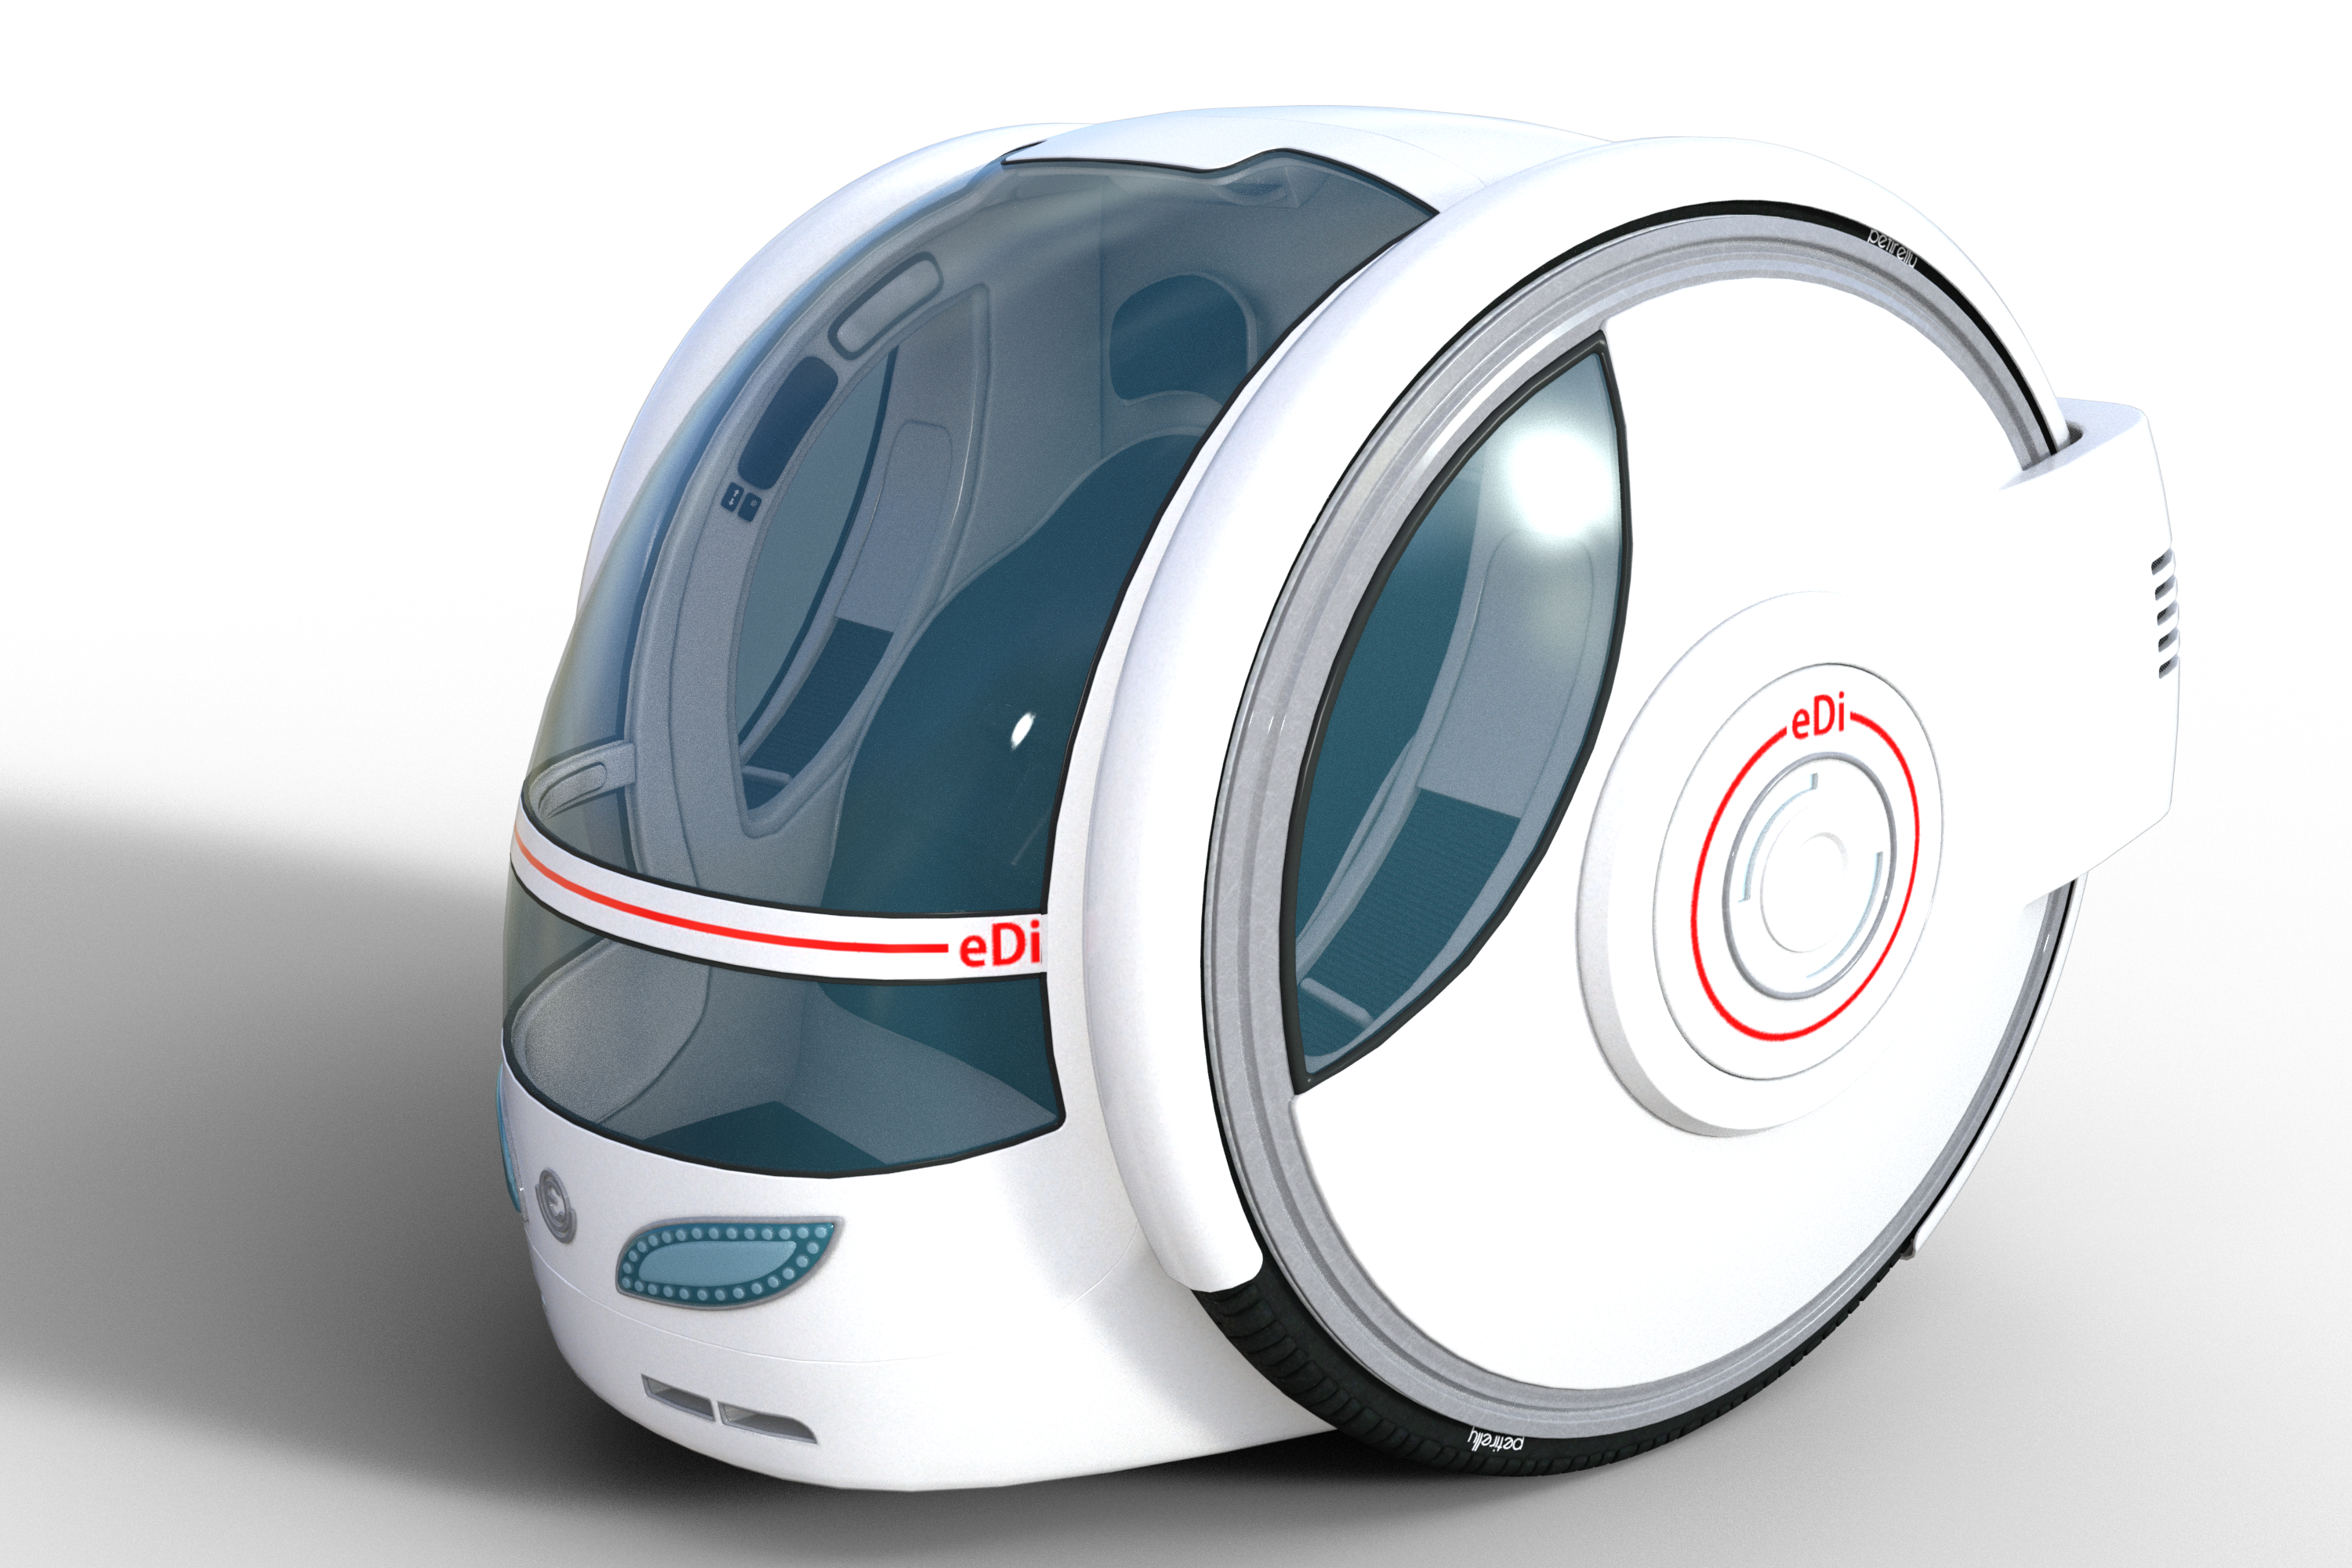
\includegraphics[width=\linewidth]{graphIII-11-mystic-art-design-pixabay-auto-2651594.png}}
Une telle illustration est donnée par les scientifiques pour imager les futurs possibles avec les avantages et les inconvénients. Leur rôle n'est alors pas de trancher mais c'est à la société toute entière qu'il appartient de faire des choix, de formuler les réactions à envisager face à des évènements inadmissibles.

\subsubsection[Collaboration homme-robot]{Collaboration homme-robot}
\label{subsub:III.3.1.2}

Le robot se rapproche de l'homme dans une fonction d'aide et d'appui, mais aussi pour observer le comportement de l'humain dans certaines circonstances et gérer des situations d'urgence.

Ces robots d'assistance commencent à investir le monde industriel sous couvert de l'appellation de « cobots ». Il s'agit d'un système qui promeut la \emph{collaboration} en l'homme et le robot. Le robot va se charger des tâches les plus dangereuses ou les plus pénibles comme soulever de lourdes charges. En revanche, l'homme possède une expertise du geste que le robot n'atteindra jamais, mais a des difficultés vis-à-vis de l'applicabilité de la tâche. Faire cohabiter ces deux approches semble relever du bon sens.

\sidegraphic[\href{https://fr.wikipedia.org/wiki/Atlas_(robot)}{Atlas} (2013), robot androïde de \textsc{Boston Dynamics}.]{\includegraphics[width=\linewidth]{graphIII-12-robot-atlas-frontview-2013.jpg}}
Dans le cas de la robotique industrielle, la législation est assez claire et bien balisée en terme de gestion des risques. Par contre, l'aspect observationnel pose des problèmes d'éthique car la machine qui aide l'homme va être capable de donner des informations sur la manière dont il effectue son travail. On peut arguer que c'est une bonne chose et que les indicateurs de performance chers à nos \textit{managers} vont être utiles au développement de l'entreprise. 
En même temps, ces indicateurs sont très souvent établis avec une machine qui n'est pas complètement au courant de l'ensemble du contexte de la réalisation de la tâche. Il peut donc y avoir des raisons objectives à faire quelque chose moins vite que d'habitude parce qu'il y a eu un facteur de complexité supplémentaire qui ne sera pas mesuré par les indicateurs. Donc, ça pose un tout petit peu de soucis d'évaluer les personnes par des machines qui n'ont pas forcément toutes les capacités pour appréhender la situation à sa juste valeur. 

En parallèle, il y a bien sûr le problème de l'observation de l'homme par la machine. Est-ce que le technicien qui fait le geste va accepter d'être surveillé par cette machine ? Qu'est-ce qu'on lui dit à ce technicien de ce que fait la machine, de ce que mesure la machine ? Dans quel objectif a-t-il accès à ces données ? Sont-elles anonymisées ? Servent-elles simplement à faire des traitements statistiques ? Est-ce qu'elles vont sortir de l'entreprise ? Tout cela relève de problèmes d'éthique sur lesquels il faudra bien un jour se pencher. 
 
\subsubsection[Enjeux de la robotique médicale]{Enjeux de la robotique médicale}
\label{subsub:III.3.1.3}

On peut également considérer le domaine de la robotique médicale où la motivation première des machines est l'assistance à la personne. L’objectif est aussi de s’adresser ici à la communauté médicale pour évaluer l'état de santé d'un patient, être capable d'observer son comportement et de signaler des situations d'urgence, comme par exemple de détecter l'apparition d'une pathologie émergente parce que le dispositif d'assistance va relever et mesurer une anomalie qui va attirer l'attention d'un médecin.

Les avantages sont là encore nombreux... Tout autant que les problèmes d'éthique. D'abord, que ce passe-t-il lorsque le dispositif d'assistance blesse le patient, par exemple une machine puissante destinée à lever des personnes ? Le risque est donc accru et pose le problème de l'acceptation. Jusqu'où tolère-t-on qu'une machine prenne en charge la mobilité d'une personne sachant que cette machine fatalement un jour présentera un défaut ?

Là encore, de même qu'en cobotique, on retrouve aussi la problématique de l'observationnel de l'individu. Certes, on part d'un bon sentiment ; on mesure des paramètres d'état de santé. Mais évidemment, ces données peuvent avoir un intérêt économique très fort auprès de personnes extérieures qui vont par exemple profiter de l'état de faiblesse des personnes âgées pour essayer de leur vendre de l'assurance-vie, de la téléassistance ou tout ce qu'on peut imaginer comme solutions dont l'efficacité reste encore à prouver mais qui présentent pour les entreprises un intérêt économique considérable. 

Donc, qu'est-il acceptable en termes d'observation ? Qu'est-ce qu'on va donner comme information au sujet qui est instrumenté ou qui utilise un objet de sa vie quotidienne pour évaluer son état ? Qu'est-ce qu'on lui dit de ce qu'on observe et en des termes suffisamment simples pour que cela soit compréhensible par tout utilisateur. Cela pose déjà un petit problème sur la sécurité des informations. Ces informations, on peut certes les anonymiser\sidenote{Voir \cref{sub:I.4}, \qnameref{chap:I}.} et on peut essayer de les crypter. Malgré tout, à un moment donné, il faudra bien les transmettre. Transmettre à qui ? Dans un cadre privilégié d'une relation médecin-patient, donc juste vers le médecin ? Plus largement, ces données ont pourtant un intérêt pour la communauté médicale puisqu'on peut observer des tas de choses sur un grand nombre d'individus. Ce faisant, cela peut aider à faire progresser des traitements en se fondant justement sur ces analyses de grandes données. Donc on est dans une espèce d’antinomie ou les données devraient être les plus confidentielles possible et, en même temps, devraient être utilisées par au moins un public très averti pour en tirer des bénéfices sur la médecine. 

Après, il y a la sécurité des transmissions. Alors d'abord, là aussi, il faut démythifier un tout petit peu ce monde hyper-connecté de manière extrêmement fiable qu'on nous présente. C'est loin d'être la réalité et il n'y a pas besoin d'aller très loin autour de soi pour trouver une zone blanche. Imaginez une personne âgée qui chute, il faut absolument transmettre cette information pour la sauver. Mais là, on peut être dans un contexte où le réseau classique d'informations ne fonctionne pas. Cela veut dire que là aussi, il faut inventer des solutions alternatives aux réseaux Wifi ou hertzien qui permettront la transmission de cette information. Donc trouver des solutions alternatives de transmission de l'information tout en garantissant la sécurité, qu'un extérieur ne puisse pas intercepter ces informations pour les exploiter de manière frauduleuse. 

De tous ces problèmes soulevés par la robotique, les experts scientifiques sont capables de voir et d'anticiper leurs avantages et leurs inconvénients, mais c'est à l'ensemble de la société, au législateur, aux citoyens de décider de ce qui sera admissible ou non. 

\printlocalglossary{13}

%\begin{jazzgraphic*}
%\includegraphics[width=\linewidth]{gerd-altmann-pixabay-finger-4785082.jpg}
%\end{jazzgraphic*}

\subsection[Informaticiens et éthique]{Informaticiens et éthique du numérique}
\label{sub:III.3.2}

Que deviendra la notion de vie privée\caution[t]<firstcolor>{%
\upshape Texte rédigé par Max \textsc{Dauchet} et publié sur \href{https://www.lemonde.fr/blog/binaire/2014/03/11/les-informaticiens-et-lethique-du-numerique/}{Binaire} --- blog du numérique du journal \textsc{Le Monde} --- le 11 mars 2014.}{\upshape Note de la rédaction}
 dans notre société numérique ? L’hypermnésie et l’hyper-connectivité du net sont-elles des facteurs d’asservissement ou de libération de l’homme ? Quelle sera notre responsabilité vis-à-vis de robots commandés par la pensée, quelle sera notre cohabitation avec les robots ? Construire des robots ressemblant à l’homme est-il tabou ? Faut-il souhaiter ou redouter le transhumain, cet hypothétique homme augmenté de capacités intellectuelles et physiques jusqu’à prendre notre relai dans l’évolution ? Peut-on sans précautions utiliser des données personnelles, génétiques ou comportementales, à des fins de recherches ?

Cet échantillon d’interrogations --- dont certaines relèvent encore de la fiction --- illustre l’ampleur et la diversité des questions éthiques que pose l’explosion du numérique.

Il serait présomptueux de vouloir traiter ici ces questions, d’autant que l’on ne peut pas en débattre entre informaticiens seulement ; le propos est plutôt d’esquisser comment le monde scientifique les aborde actuellement. Au delà des seuls spécialistes, l’accent est mis sur la nécessaire approche décloisonnée des questions éthiques et la nécessaire inscription de celles-ci dans l’espace public.

\overparagraph*{Éthique et déontologie}

\sidegraphic{\includegraphics[width=\linewidth]{the-economist-2009.png}}
En gros l’éthique --- qu’elle soit générale ou appliquée à un domaine --- relève d’abord de la philosophie et l’humain est en son centre. L’éthique se définit classiquement comme la science de la morale.

La déontologie, qui n’est pas notre sujet ici, définit de manière plus opérationnelle les pratiques d’une profession, en accord avec l’éthique et le droit. La plus connue est la déontologie médicale. En informatique, le \textsc{Cigref} (grandes entreprises utilisatrices) et le \textsc{Syntec} (SSI) ont défini leur code de déontologie. La déontologie engage comme le serment d’Hippocrate. L’\textsc{Anr}, agence nationale de projets scientifiques, affiche pour sa part une charte qui énumère les éléments suivants :
\setlength{\columnsep}{12pt}
\begin{multicols}{2}
\begin{itemize}
\item Développer une recherche sérieuse et fiable ; 
\item Honnêteté dans la communication ; 
\item Objectivité ; 
\item Impartialité, indépendance ; 
\item Ouverture et accessibilité ; 
\item Devoir de précaution ; 
\item Équité dans la fourniture de références et de crédits ; 
\item Responsabilité vis-à-vis des scientifiques et chercheurs à venir.
\end{itemize}
\end{multicols}

Dans le monde anglo-saxon, on parle plus volontiers d’intégrité (\textit{integrity}) qui met l’accent sur la responsabilité individuelle de comportement. Le comité d’éthique du \textsc{Cnrs} (\textsc{Comets}) vient dans cet esprit d’éditer un guide pour promouvoir une recherche intègre et responsable.

\overparagraph*{Une approche scientifique nécessairement ouverte}

Partout, les réflexions éthiques mobilisent le regard croisé des philosophes, historiens, sociologues, juristes voire économistes. On peut même dire « qu’élargir ses horizons » est inhérent à la démarche éthi\-que, car on ne peut en général pas isoler les réflexions sur une science ou une technologie. Par exemple, en informatique, les considérations sur le \textit{Big Data} ou sur l’anonymat ne peuvent être considérées que dans le contexte sociétal.

\overparagraph*{Des sujets incontournables}

Dans le but louable de financer équitablement les cultes, les Pays-Bas avaient mis en cartes perforées IBM les données confessionnelles de leur population dès les années trente, ce qui servit en 1940 les funestes desseins des envahisseurs nazis. Notons que ce pays intègre maintenant tout particulièrement la préoccupation éthique dans ses programmes scientifiques. Certes, on ne peut pas incriminer les seules technologies, la délation par la peur et l’oppression est arrivée ailleurs au même résultat avec du papier et des crayons seulement. Il reste qu’au-delà des controverses, on voit que l’on peut difficilement se laver les mains de tels sujets : \textit{in fine}, il s’agit des rapports entre la démocratie et les totalitarismes et, de l’avenir de notre monde.

Depuis le procès des médecins de Nuremberg et maintenant avec les possibilités ouvertes par la biologie et la médecine, la bioéthique occupe le devant de la scène en éthique appliquée. Cependant les débats éthiques s’élargissent et la sécurité alimentaire, l’environnement et le numérique suscitent à leur tour des questionnements. Ainsi au niveau européen le réputé appel à projets individuels de l’\textit{European Research Council} (ERC) compte 105 occurrences de “\textit{ethic(s)}” ! De plus, les candidats doivent remplir un questionnaire éthique de vingt-six items, dont une douzaine est susceptible de concerner le numérique, notamment à travers l’usage de données personnelles (dont génétiques ou biométriques), les neurosciences, les technologies pour la santé, l’usage militaire ou encore la vie privée (la surveillance et maintenant la sous-veillance, qui consiste en la possibilité pour chacun de mettre instantanément sur le \textit{Net} tout ce qu’il perçoit ou que son \textit{smartphone} capte des personnes qu’il croise).

\overparagraph*{Des perceptions variables de par le monde}

Une vision de l’homme inspirée des religions révélées, celles des fils d’Abraham, peut percevoir le transhumanisme comme une transgression. Un asiatique influencé par le shintoïsme peut par contre concevoir l’homme comme participant à un tout dans un continuum entre la vie, la nature et l’artefact et ne manifester aucune appréhension à l’égard des humanoïdes. Dans nos sociétés, la confiance en la science comme vecteur de progrès s’effrite parfois face à l’ambivalence des technologies qui envahissent notre quotidien. Ainsi on peut voir dans les technologies numériques un facilitateur d’épanouissement et de démocratie ou, à l’opposé, un instrument mu par le profit qui accroît les inégalités entre les hommes. Les compromis entre respect de la vie privée et sécurité sont perçus différemment selon les continents ou les aspirations politiques... Plus généralement, une étude norvégienne de 2010\sidenote{ROSE, \textit{Relevance Of Science Education}.} portant sur trente-quatre pays représentatifs de la diversité de la planète met en évidence de grandes diversités de perception des sciences et des technologies selon les continents, les cultures, la richesse par habitant ou encore le genre. Un maillage sans frontières des réflexions est donc nécessaire afin d’avoir pleinement conscience de la relativité des préconisations que l’on peut formuler à l’attention d’une nation ou d’une communauté --- ainsi en Californie les journaux parlent le plus souvent de l’informatique pour souligner de nouveaux systèmes, des réussites, alors qu’en France on va insister sur les risques de pédophilies.

\overparagraph*{Un paysage en construction}

Face à ces enjeux les initiatives se multiplient, principalement sous l’impulsion des États-Unis d’une part et de l’Europe d’autre part. Sur le plan scientifique, la bioéthique naturellement, mais aussi l’environnement et la sécurité alimentaire provoquent des débats de société, davantage que le numérique, car ces secteurs sont perçus comme conditionnant de manière intrusive le devenir biologique de notre espèce.

\paragraph*{Les comités d’éthique scientifique}
Ce sont généralement des instances consultatives, indépendantes, que l’on peut saisir ou qui s’auto-saisissent de sujets éthiques, et qui fournissent des préconisations. Ils ont un rôle de réflexion et sensibilisation amont.

En Europe, l’\textit{European Group of Ethics} (EGE) joue ce rôle sur tout le spectre scientifique. La Commission Européenne est certes prolixe en tous domaines, mais on soulignera quand même l’abondance de la documentation sur l’éthique en général, et sur le numérique en particulier. Cette abondance semble viser davantage la sensibilisation des chercheurs que la construction d’une vision proprement européenne.

En France, le plus ancien et le plus en vue est le \textsc{Ccne}, créé en 1983 à l’initiative de François \textsc{Mitterrand}. Ce comité est placé auprès du Premier ministre, et sa composition garantit la représentation des grands courants philosophiques et religieux. Le \textsc{Cnrs} dispose pour sa part depuis 1994 du \textsc{Comets}. L’\textsc{Inra} et le \textsc{Cirad} ont fusionné leurs comités.

Concernant l’informatique, la \href{http://cerna-ethics-allistene.org/}{\textsc{Cerna}} (Commission de réflexion sur l’éthique de la recherche en sciences et technologies du numérique d’Allistene) a été créée fin 2012 sous l’impulsion de l'\textsc{Inria} et du \textsc{Cnrs} par Allistene, l’alliance des sciences et technologies du numérique qui réunit le \textsc{Cea}, la \textsc{Cge}, le \textsc{Cnrs}, la \textsc{Cpu}, \textsc{Inria} et l’Institut \textsc{Mines-Télécom}. Le point de vue y est celui de la recherche et non des usages.

Il s’ajoute encore au paysage des groupes de travail qui émergent à l’initiative d’établissements ou de groupes d’établissements, comme par exemple le groupe Prométhos en éthique de l’innovation sur le plateau de Saclay.

\paragraph*{Les comités opérationnels d’établissement}
Ils trai\-tent les questions engageant leur responsabilité à travers des projets ou la déontologie des personnels.

\paragraph*{Les instances de validation et certification (respect de normes éthiques)}
De plus en plus d’institutions demandent une certification de conformité éthique des projets de recherche attestée par un \textit{Institutional Review Board} (IRB), notamment pour les recherches impliquant l’homme.

\paragraph*{Les espaces de débat public}
La France dispose depuis 1995 d’une \href{https://www.debatpublic.fr/}{Commission nationale du débat public} (\textsc{Cndp}), créée dans le cadre de la loi relative au renforcement de la protection de l’environnement, dite loi Barnier. Cette commission, aux consultations fort diverses, a notamment (mal)traité des nanotechnologies en 2010.

À un niveau intermédiaire entre le débat public et le cénacle de spécialistes, on peut citer les espaces éthiques régionaux qui se mettent en place à l’initiative du \textsc{Ccne}. Centrés sur la pratique hospitalière, ils associent des représentants des usagers.

Notons aussi que face au trouble suscité par la biologie de synthèse, le ministère de l’enseignement supérieur et de la recherche a confié en 2012 au \textsc{Cnam} la création d’un observatoire de la biologie de synthèse, chargé d’informer le grand public et d’échanger avec lui.

\paragraph*{Les conférences et symposiums scientifiques}
Il est naturel que des manifestations scientifiques accompagnent la montée des préoccupations éthiques, dans le numérique comme ailleurs. Ainsi l’IEEE, maintenant association internationale des professionnels du secteur numérique et dont les racines remontent à 1884 et l’avènement de la fée électricité, lance l’année prochaine un symposium sur l’éthique appelé à devenir annuel.

Deux conférences internationales de recherche sont consacrées depuis une vingtaine d’années aux différents aspects éthiques liés à l’informatique, CEPE et ETHICOMP. À l’initiative de la \textsc{Cerna}, elles se tiendront cette année conjointement et pour la première fois en France.

D’une manière générale, les Français sont peu présents dans ce genre de manifestation. Ainsi, lors de la \textit{Third World Conference on Research Integrity} (WCRI) qui s’est tenue en 2013 à Montréal, il n’y avait que quatre français sur 500 participants. Ce manque d’appétence de notre monde académique est peut-être dû à la faible reconnaissance dans notre pays des investissements dans les questions éthiques et plus généralement les questions interdisciplinaires. Peut-être aussi que le regard fixé dans le rétroviseur sur notre rôle phare du temps des Lumières, nous percevons avec circonspections les nouveaux espaces éthiques qu’ouvrent les technosciences. Nuançant ce dernier propos, de nouveaux lieux de réflexions émergent dans notre pays, notamment au sein d’associations comme la \href{https://fing.org/}{\textsc{Fing}} (Fondation Internet nouvelle génération), \href{https://www.renaissancenumerique.org/}{Renaissance numérique}, la \href{https://www.laquadrature.net/}{Quadrature du net}. Par ailleurs, l’\href{https://afia.asso.fr/}{\textsc{Afia}} (Association française d’intelligence artificielle) a consacré un récent bulletin à un « Dossier Éthique et IA », et la \href{https://www.societe-informatique-de-france.fr/}{\textsc{Sif}} (Société informatique de France) a reproduit une première version du présent propos dès le numéro deux de son bulletin intitulé 1024.

\begin{jazzgraphic*}
\includegraphics[width=\linewidth]{gerd-altmann-pixabay-finger-4785082.jpg}
\end{jazzgraphic*}

En conclusion, il importe que les scientifiques contribuent aux débats sur l’éthique des nouvelles technologies, et du numérique en particulier, faute de quoi les espaces laissés en friches pourraient être investis par des obscurantistes ou des aventuriers. Nous devons aussi veiller dans notre pays à dépasser nos vieilles habitudes de « s’affronter d’abord, débattre ensuite », car aborder les sujets éthiques en termes de pro- versus anti-technologies nous ferait passer tragiquement à côté du sujet. Et pour cela sensibilisons, informons, formons à commencer par la jeunesse.

\begin{gofurther}
\begin{itemize}\jazzitem
\item \href{https://www.lemonde.fr/blog/binaire/2015/03/02/des-robots-et-des-humains/}{Des robots et des humains}, Jean-Pierre \textsc{Merlet}, \textsc{Interstices}, 20 février 2015 et \textsc{Binaire}, 02 mars 2015 ;
\item \href{https://www.podcastscience.fm/emission/2016/07/11/podcast-science-266-informatique-et-ethique-avec-serge-abiteboul-et-gilles-dowek/}{Informatique et éthique}, Serge \textsc{Abiteboul} et Gilles \textsc{Doweck}, Podcast Science \#166, 11 juillet 2016 (160 minutes) ;
\item \href{https://www.lemonde.fr/sciences/article/2016/06/23/tuer-un-pieton-ou-sacrifier-le-passager-le-dilemme-macabre-des-voitures-autonomes_4956924_1650684.html}{Le dilemme macabre de la voiture automatique : tuer un piéton ou le passager ?} David \textsc{Larousserie}, \textsc{le Monde Science et Techno}, 23 juin 2016 ;
\item \href{https://www.lemonde.fr/blog/binaire/2016/09/16/laurence-devillers-lempathie-des-robots/}{L'emphatie des robots}, où comment démystifier cette idée de personnification des robots, tout en montrant comment simuler cela de manière très sophistiquée, Laurence \textsc{Devillers}, Binaire, 16 septembre 2016  ;
\item \href{http://glorieusefrance.fr/limpact-de-la-revolution-robotique-sur-le-droit/}{Quel impact de la révolution robotique sur le droit français ?} texte d'analyse, Alexandre \textsc{Mandil}, \textsc{Glorieuse France droit \& intelligence économique}, 21 février 2016.
\end{itemize}
\end{gofurther}



%----------
\section[\textit{Deap learning}]{\textit{Deap learning}}
\label{sec:III.4}

L'apprentissage automatique (\textit{machine learning}) correspond à des algorithmes qui ajustent les paramètres de leurs calculs en fonction des exemples qui leur sont donnés. Cela permet d'adapter leur fonctionnement aux données fournies. L'apprentissage profond (\textit{deep learning}) est une architecture qui associe en cascade plusieurs couches d'algorithmes de ce type pour hiérarchiser le problème et obtenir des performances bien plus importantes. Ce n'est pas simple ! Mais à expliquer, plus sûrement...


\subsection[Comprendre le \textit{deap learning}]{Comprendre le \textit{deap learning}}
\label{sub:III.4.1}

Les concepts du \textit{machine learning}\caution[t]<secondcolor>{%
David \textsc{Louapre}, normalien et docteur en physique théorique, est chercheur dans l'industrie des matériaux. Passionné de culture scientifique, son parcours lui a\linebreak permis de s’intéresser à de nombreux domaines de la science (physique fondamentale, mathématiques appliquées,\linebreak physico-chimie des matériaux, thermi\-que, mécanique, etc.). Il se qualifie de «~responsable R{\&}D (le jour), vulgarisateur scientifique (la nuit) ».}{À propos de l'intervenant}
 et du \textit{deap learning} sont directement abordés par la vidéo de « Science étonnante » proposée par David \textsc{Louapre}. Les contenus sont issus d'un livre de vulgarisation scientifique : « \href{https://editions.flammarion.com/Catalogue/hors-collection/sciences/mais-qui-a-attrape-le-bison-de-higgs}{Mais qui a attrapé le bison de \textsc{Higgs} ?} aux éditions Flammarion. Un \href{https://scienceetonnante.com/2016/04/08/le-deep-learning/}{billet} vient compléter la vidéo en abordant les concepts sous-jacents n'ayant pas été intégrés à la vidéo.

On peut suivre son partage de grains de « science étonnante » sur son \href{https://scienceetonnante.com/}{blog} et son canal vidéo.

\begin{marginvideo}
	[\label{vid:III.5}Deap learning.]%
	\vspace{2cm}%
	\movie[width=\marginparwidth,showcontrols]%
		{\includegraphics[width=\marginparwidth]{./Images/Pictograms/film-strip-dark-electric-blue.png}}%
		{./Videos/Chapter03/vidIII-04-deep learning-HD.mp4}%
	\launchvideo{./Videos/Chapter03/vidIII-04-deep learning-HD.mp4}
\end{marginvideo}


\printlocalglossary{14}


\subsection[Apprentissage automatique]{Apprentissage automatique : pas à pas !}
\label{sub:III.4.2}

\overparagraph*{Apprentissage automatique dites-vous ?}

Il est très probable\caution[t]<firstcolor>{%
\upshape Texte rédigé\parnote{Les éléments liés à une actualité ont été enlevés pour alléger le texte.} par Colin \textsc{de la Higuera} et publié sur \href{https://www.lemonde.fr/blog/binaire/2015/06/23/pasapas/}{Binaire} --- blog du numérique du journal \textsc{Le Monde} --- le 23 juin 2015.\parnotes}{\upshape Note de la rédaction}
 qu’à l’heure où vous lisez ces lignes, vous aurez utilisé le résultat d’algorithmes d’apprentissage automatique plusieurs fois aujourd’hui : votre réseau social favori vous a peut-être proposé de nouveaux amis et le moteur de recherche a jugé certaines pages pertinentes pour vous mais pas pour votre voisin. Vous avez dicté un message sur votre téléphone portable, utilisé un logiciel de reconnaissance optique de caractères, lu un article qui vous a été proposé spécifiquement en fonction de vos préférences et qui a peut-être été \href{https://interstices.info/la-traduction-automatique-statistique-comment-ca-marche/}{traduit automatiquement}.

Et même sans avoir utilisé un ordinateur, vous avez été peut être écouté les informations : or la météo entendue ce matin, la plupart des transactions et des décisions boursières qui font et défont une économie, et de plus en plus de diagnostics médicaux reposent bien plus sur les qualités de l’algorithme que sur celles d’un expert humain incapable de traiter la montagne d’informations nécessaire à une prise de décision pertinente.

De tels algorithmes ont appris à partir de données, ils font de l’apprentissage automatique. Ces algorithmes construisent un modèle à partir de données dans le but d’émettre des prédictions ou des décisions basées sur les \href{https://en.wikipedia.org/wiki/Machine_learning}{données}.

\overparagraph*{Mais depuis quand confie t’on cela à des algorithmes ?}

L’idée de faire apprendre la machine pour lui donner des moyens supplémentaires est presque aussi ancienne que l’informatique. C’est Alan \textsc{Turing} lui-même qui après avoir, en 1936, jeté les bases conceptuelles du calcul sur machine, donc de l’ordinateur, allait s’intéresser à cette possibilité. Il envisage en 1948 des « \textit{learning machines} » susceptibles de construire elles-mêmes leurs propres codes.

\sidegraphic{\includegraphics[width=\linewidth]{France-in-XXI-Century-School.jpg}}%
Tout compte fait, c’est une suite logique de cette notion de machine de calcul dite universelle (c’est-à-dire qui peut exécuter tous les algorithmes, comme le sont nos ordinateurs ou nos \textit{smartphones}). Puisque le code d’une machine, le programme, n’est qu’une donnée comme les autres, il est raisonnable d’envisager qu’un autre programme puisse le transformer. Donc pourquoi ne pas apprendre de nouveaux program\-mes à partir de données ?

Vue la quantité astronomique de donnée, on peut apprendre simplement en les analysant. Mais les chercheurs se sont rendus compte que dans ce contexte, un programme qui se comporte de manière déterministe n’est pas si intéressant. C’est le moment où on découvre les limites de ce qui est \href{https://www.lemonde.fr/blog/binaire/2015/06/17/decidable-indecidable/}{décidable ou indécidable} avec des algorithmes. Il faut alors introduire une autre idée : celle d’exploration, de recours au hasard, pour que de telles machines soient capables de comportements non prévus par leur concepteur.

Il y a donc une rupture entre programmer, c’est-à-dire imaginer et implémenter un calcul sur la machine pour résoudre un problème, et doter la machine de la capacité d’apprendre et de s’adapter aux données. De ce fait, on ne peut plus systématiquement prévoir un comportement donné, mais uniquement spécifier une classe de comportements possibles.

%\overparagraph*{Alors... Ça y est ? Nous avons créé de l’intelligence artificielle (IA) ?}
\overparagraph*{Alors... Ça y est ? L’intelligence artificielle est créée ?}

C’est une situation paradoxale, car le terme d’IA veut dire plusieurs choses. Quand on évoque l’intelligence artificielle, on pense à \emph{appren\-dre}, \emph{évoluer}, \emph{s’adapter}. Ce sont des termes qui font référence à des activités cognitives qui nous paraissent un ordre de grandeur plus intelligentes que ce que peut produire un calcul programmé.

Et c’est vrai qu’historiquement, les premiers systèmes qui appren\-nent sont à mettre au crédit des chercheurs en IA. Il s’agissait de repousser les frontières de la machine, de tenter de reproduire le cerveau humain. Les systèmes proposés devaient permettre à un robot d’être autonome, à un agent de répondre à toute question, à un joueur de s’améliorer défaite après défaite.

Mais, on s’accorde à dire que l’intelligence artificielle n’a pas tenu \href{http://www.scilogs.fr/intelligence-mecanique/lintelligence-artificielle-naura-pas-lieu/}{ses promesses}. Pourtant ces algorithmes d’apprentissage automatique, une de ses principales composantes, sont bel et bien présents un peu partout aujourd’hui. Et ceci, au delà, du fait que ces idées sont à la source de nombreuses pages de science-fiction.

\begin{jazzgraphic*}
\includegraphics[width=\linewidth]{gerd-altmann-pixabay-web-3706562.jpg}
\end{jazzgraphic*}

C’est peut-être notre vision de l’intelligence qui évolue avec la progression des sciences informatiques. Par exemple, pour gagner aux\linebreak échecs il faut être bougrement intelligent. Mais quand un algorithme qui se contente de faire des statistiques sur un nombre colossal de parties défait le champion du monde, on se dit que finalement l’ordinateur a gagné « bêtement ». Ou encore: une machine qui rassemble toutes les connaissances humaines de manière structurée pour que chacun y accède à loisir sur simple demande, est forcément prodigieusement intelligente. Mais devant \textsc{Wikipédia}, qui incarne ce rêve, il est clair que non seulement une vision encyclopédique de l’intelligence est incomplète, mais que notre propre façon de profiter de notre intelligence humaine est amenée à évoluer, comme nous le rappelle Michel Serres.

\overparagraph*{Passionnant ! Mais [que se passe-t-il maintenant] ?}

L’apprentissage automatique est maintenant devenu une matière enseignée dans de nombreux cursus universitaires. Son champ d’application augmente de jour en jour : dès qu’un domaine dispose de données, la question de l’utilisation de celles-ci pour améliorer les algorithmes du domaine se pose systématiquement.

Mais c’est également un sujet de recherche très actif. Les chercheurs du monde entier, [étudient] parmi d’autres, les questions à suivre.
\begin{jazzitemize}
\item Une famille d’algorithmes particulièrement efficace aujourd’hui permet d’effectuer un apprentissage profond (« \textit{deep learning} »). De tels algorithmes simulent une architecture complexe, formées de couches de neurones artificiels, qui permettent d’implémenter des calculs distribués impossibles à programmer explicitement.
\item L’explosion du phénomène du \textit{big data} est un levier. Là où dans d’au\-tres cas, la taille massive des données est un obstacle, ici, justement, c’est ce qui donne de la puissance au phénomène. Les algorithmes, comme ceux d’apprentissage profond, deviennent d’autant plus performants quand la quantité de données augmente.
\item Nul doute que des modèles probabilistes de plus en plus sophistiqués seront discutés. L’enjeu aujourd’hui est d’apprendre en mettant à profit le hasard pour explorer des solutions impossibles à énumérer explicitement.
\item la notion de prédiction sera une problématique majeure pour ces chercheurs qui se demanderont comment utiliser l’apprentissage sur une tâche pour prévoir comment en résoudre une autre.
\item Les applications continueront à être des moteurs de l’innovation dans le domaine et reposent sur des questions nouvelles venant de secteurs les plus variés : le traitement de la langue, le médical, les réseaux sociaux, les villes intelligentes, l’énergie, la robotique...
\end{jazzitemize}

%\begin{jazzgraphic}
%\includegraphics[width=\linewidth]{France-in-XXI-Century-School.jpg}
%\end{jazzgraphic}

Il est possible --- et souhaitable --- que les chercheurs trouvent également un moment pour discuter des questions de fond, de société, soulevées par les résultats de leurs travaux. Les algorithmes appren\-nent aujourd’hui des modèles qui reconnaissent mieux un objet que l’œil humain, qui discernent mieux les motifs dans des images médicales que les spécialistes les mieux entraînés. La taille et la complexité des modèles en font cependant parfois des boîtes noires : la machine peut indiquer la présence d’une tumeur sans nécessairement pouvoir expliquer ce qui justifie son diagnostic : sa « décision » reposera peut-être sur une combinaison de milliers de paramètres, combinaison que l’humain ne connaît pas.

Or, quand votre médecin vous explique qu’il serait utile de traiter une pathologie, il vous explique pourquoi. Mais quand la machine nous proposera de subir une intervention chirurgicale, avec une erreur moindre que le meilleur médecin, sans nous fournir une explication compréhensible, que ferons-nous ? [...]

%\overparagraph*{Et... Pour en savoir plus sur tout cela ?}

%C’est tout à fait passionnant et... Très sérieux.

%Pour l’apprentissage automatique, nous allons vous lancer un défi. Revenez sur \textsc{Binaire} [] et nous allons oser vous expliquer ce qui se trouve sous le capot : \href{https://www.lemonde.fr/blog/binaire/2015/06/29/lapprentissage-automatique-le-diable-nest-pas-dans-lalgorithme/}{comment \emph{la machine construit des modèles et les exploite ensuite}}. Et vous verrez que si un sorcier ou une sorcière avait osé proposé une telle machine il y a quelques siècles, c’est sur un bûcher qu’elle ou il aurait fini.

%Et pour mieux comprendre toutes les autres facettes de la science informatique \href{https://www.lemonde.fr/blog/binaire/2015/06/12/science-informatique-dites-vous-deux-revues-et-un-blog-a-votre-service/}{deux revues et un blog sont à votre service}. \href{https://interstices.info/comment-donner-un-sens-a-limage-numerique/}{Comment donner un sens à l’image numérique ?} \href{https://interstices.info/la-traduction-automatique-statistique-comment-ca-marche/}{Comment marche la traduction automatique ?}  En quoi notre cerveau est plus rapide que nous pour reconnaître un objet ? Les nouveaux liens entre \href{https://interstices.info/des-robots-et-des-humains/}{robots et des humains} ? Voici quelques exemples de ce que vous y trouverez.


\begin{tcolorbox}[title={Bibliographie circonstanciée}, toprule=0pt, leftrule=0pt, rightrule=0pt, arc=0pt,
                  fonttitle=\scshape\boxtitlefont,
                  colbacktitle=white, coltitle=fourthcolor, colframe=fourthcolor, colback=fourthcolor!10,
                  breakable, enhanced jigsaw]
\begin{jazzitemize}
\item \textit{Probabilistic machine learning and artificial intelligence}, Zoubin \textsc{Ghahramani}. Nature 521, pp. 452–459.
\item \textit{Apprentissage artificiel}, Antoine \textsc{Cornuéjols} et Laurent \textsc{Miclet}, \textsc{Eyrolles}, Collection Algorithmes, 2\frup{e} édition, juillet 2011.
\item \textit{Intelligence artificielle}, Stuart \textsc{Russel} et Peter \textsc{Norvig}. \textsc{Pearson Education}, 2010.
\item \textit{Machine Learning}, Peter \textsc{Flach}, \textsc{Cambridge University Press}, November 2012.
\item \textit{Computing machinery and intelligence}, Alan M. \textsc{Turing}, \textsc{Mind}, 59, pp. 433-460, 1950.
\item \href{https://interstices.info/lapprentissage-profond-une-idee-a-creuser/}{\textit{L’apprentissage profond : une idée à creuser ?}}  Ikram \textsc{Chraibi Kaadoud} et Thierry \textsc{Viéville}, \textsc{Interstices}, 29 avril 2016.
\item \href{https://www.lemonde.fr/blog/binaire/2015/06/29/lapprentissage-automatique-le-diable-nest-pas-dans-lalgorithme/}{L’apprentissage automatique : le diable n’est pas dans l’algorithme}, Philippe \textsc{Preux}, Marc \textsc{Tommasi}, Thierry \textsc{Viéville} et Colin \textsc{de la Higuera}, Binaire, 29 juin 2015.
\item \href{https://interstices.info/comment-donner-un-sens-a-limage-numerique/}{Comment donner un sens à l’image numérique ?}  Jean \textsc{Ponce}, \textsc{Interstices}, 9 décembre 2014.
\end{jazzitemize}
\end{tcolorbox}

\begin{gofurther}
\begin{itemize}\jazzitem
\item \href{https://www.ted.com/talks/fei_fei_li_how_we_re_teaching_computers_to_understand_pictures?language=fr}{Comment apprendre aux ordinateurs à comprendre des images}, Fei-Fei \textsc{Li}, conférence TED --- \textit{Technology}, \textit{Entertainment}, \textit{Design} ---, 2015 ;
\item \href{https://www.college-de-france.fr/site/yann-lecun/inaugural-lecture-2016-02-04-18h00.htm}{Conférence inaugurale} et \href{https://www.college-de-france.fr/site/yann-lecun/_audiovideos.htm}{cours} au Collège de France, Yann \textsc{LeCun}, 2015-2016.
\end{itemize}
\end{gofurther}



%----------
\section[Que faire de ces ressources ? Quiz]{Que faire de ces ressources ? Autoévaluation}
\label{sec:III.5}

Les questionnaires\caution[t]<firstcolor>{%
La présentation des quiz du document\linebreak suit plus ou moins celle de la platefor\-me \textsc{Fun-Mooc}. La fonctionnalité manquante --- pas encore implémentée dans l'extension de style \LaTeX{} usitée --- est relative à la comptabilisation des points et à leur enregistrement. Aussi, il appartient au lecteur de jouer le jeu dans l'auto\-évaluation de ses connaissances.}{Note de la rédaction}
à choix multiple%
\parnote{De manière traditionnelle en \textsc{Ihm}, lorsqu'une seule réponse est correcte, les propositions sont précédées d'un cercle à cocher (\emph{radio button}) ; en revanche, dans le cas de plusieurs solutions possibles, il s'agit de carrés (\emph{check box}). En outre, après validation des réponses (« Vérifier »), leur explication s'affiche en marge ou infobulle (« Afficher la réponse »).}
--- QCM --- à suivre clôturent le présent chapitre \qnameref{chap:III} et correspondent à chaque sujet qui y est abordé.
\parnotes

\vspace*{6pt}

\begin{quiz}[title={Robotique et intelligence artificielle}]
\begin{quizquestion*}[b]{3}{1,2,4}{Intelligence(s) artificielle(s)}
<C'est bien le fait que des méthodes numériques ou symboliques très différentes, s'appliquent selon les cas, de manière très efficace à des problèmes ciblés (reconnaissance de la parole, jeu d'échecs, etc.) mais sans que leur assemblage puisse constituer une intelligence au sens humain du terme, qui justifie l'usage du pluriel.
C'est aussi un moyen d'éviter de lancer de faux débats putatifs sur d'hypothétiques êtres artificiels de science fiction.>
On parle aujourd'hui d'intelligences artificielles au pluriel, plutôt que «~d'une » intelligence artificielle.
Que signifie cette formulation ?
\points{1}
	\mcqproposal{Le fait que les robots et les bots logiciels dotés d'une intelligence artificielle identique à l'intelligence humaine se multiplient.} %autour de nous
	\mcqproposal{Le fait qu'il y ait plusieurs niveaux dans l'intelligence artificielle, comme dans le règne animal.}
	\mcqproposal{Le fait que des méthodes radicalement différentes résolvent des problèmes très précis de manière cloisonnée.}
	\mcqproposal{C'est une simple typo qui a fini par faire le \textit{buzz}.}
\end{quizquestion*}

\begin{quizquestion}[b]{1,3}{2,4}{Intelligence(s) artificielle(s)}
<C'est bien le fait que les cobots sont des robots en interaction avec les humains au quotidien qui change la donne, et il s'agit bien, sans les personnifier, de les considérer comme des sujets de droit (de manière similaire à une association ou une structure qui est une « personne morale »).>
Pourquoi l'arrivée de cobots change-t-il la donne juridiquement ?
Donner les deux réponses exactes.
\points{1}
	\mcqproposal{De par leur interaction avec les humains au quotidien.} 
	\mcqproposal{Car dotés d'une intelligence artificielle, ils deviennent des êtres à part entière.}
	\mcqproposal{De même que pour une « personne morale », le droit est plus clair en considérant les cobots comme sujet (et non objet) de droit.}
	\mcqproposal{Par définition, puisque le terme cobot veut dire robot conscient.}
\end{quizquestion}

\begin{quizquestion*}[b]{2}{1,3}{{\itshape Deap learning}}
<C'est justement la mise à disposition d'un très grand nombre de données qui a permis à ces algorithmes d'ajuster la foule de paramètres qui les caractérisent, surtout dans le cas d'images.>
La puissance du \textit{deep learning} est de pouvoir apprendre tous les paramètres des différentes couches de calcul qui permettent de calculer une sortie à partir des entrées (par exemple étiqueter une image).
Mais qu'en est-il des données à fournir ?
\points{1}
	\mcqproposal{Ce qui est remarquable c'est qu'un tout petit ensemble de données suffit à cet apprentissage automatique.}
	\mcqproposal{Cela ne fonctionne que sur de très grands ensembles de données.}
	\mcqproposal{Si les données sont des images, une ou deux images suffisent, sinon il faut beaucoup de données.}
\end{quizquestion*}

\begin{quizquestion}<tooltip>[b]{1,3,4}{2,5}{Robot}
<Rendez-vous sur \href{https://fr.wikipedia.org/wiki/Robot}{\textsc{Wikipédia}}, la page a des éléments bien établis à partir de sources bien identifiées.>
L'origine du mot « robot » n'est pas anodine, elle montre un lien avec un vrai mythe humain.
Quelles sont les trois réponses exactes ?
\points{1}
	\mcqproposal{Cela vient du tchèque tchèque « \textit{robota} » qui signifie « travail, besogne, corvée », esclave en fait.} 
	\mcqproposal{C'est Isaac \textsc{Azimov} qui a créé le terme en même temps qu'il définissait les lois de la robotique.}
	\mcqproposal{Le mot a été employé pour la première fois dans une pièce de théâtre en 1920.}
	\mcqproposal{Le mythe initial fait référence à un être artificiel organique.}
	\mcqproposal{En fait, cela vient du français rabot et correspond au premier rabot automatisé, dans une scierie des Vosges en 1869.}
\end{quizquestion}

\begin{quizquestion*}[b]{2}{1}{Marche bipède}
<La réponse est affirmative et conduit à comprendre qu'un système dit « intelligent », ici avec un comportement sophistiqué qui peut réagir de manière pertinente en fonction d'événements externe, construit son fonctionnement par l'interaction de son anatomie avec l'environnement tout autant que par ses processus algorithmiques internes.
Cette remarque conduit à penser que l'intelligence biologique est incarnée, c'est-à-dire n'aurait pas d'existence effective si le cerveau n'était pas en interaction avec un corps et son environnement.>
Est-il possible de simuler une forme de marche bipède sur un plan incliné avec un dispositif purement mécanique sans moteur, ni aucun contrôleur électronique ou informatique ?
Cocher la réponse exacte.
\points{1}
	\mcqproposal{Évidemment non, compte-tenu de la complexité de la tâche !}
	\mcqproposal{En fait oui, c'est un comportement émergent qui résulte des interactions de la mécanique avec l'environnement.}
\end{quizquestion*}

\begin{quizquestion*}[b]{3}{1,2,4}{Environnement robotisé}
<Il semble s'avérer que ce soit les objets du quotidien, mis en réseaux et dotés de processeurs, qui vont rendre \textit{smart}\linebreak (terme anglais qui traduit intelligence mécanique tout en évitant l'amalgame avec l'intelligence humaine) l'électro-ménager, les véhicules, etc.
Cela lève\linebreak un double risque préoccupant : l'augmentation considérable de notre dépendance à ces technologies (saurons-nous toujours conduire manuellement une voiture dans quelques années ?) et l'impact environnemental qui ne cesse de croître jusqu'à une probable rupture.>
Notre environnement va être de plus en plus robotisé. Quelle forme tangible va prendre cette robotisation à grande échelle ?
Choisir la réponse la plus plausible dans l'état actuel de nos connaissances.
\points{1}
	\mcqproposal{Des robots humanoïdes, qui seront à notre service.}
	\mcqproposal{Cela n'arrivera jamais, tout ça ne marche que dans les labos.}
	\mcqproposal{Ce sont les objets du quotidien eux-mêmes qui vont se doter de processus algorithmiques sophistiqués.}
	\mcqproposal{Ils sont déjà là, moi-même, n'en suis-je pas une ou un ?}
\end{quizquestion*}
\end{quiz}
